\documentclass[a4paper, 12pt]{article}
% packages
\usepackage{amssymb}
\usepackage[fleqn]{mathtools}
\usepackage{tikz}
\usepackage{enumerate}
\usepackage{bussproofs}
\usepackage{xcolor}
\usepackage[margin=1.3cm]{geometry}
\usepackage{logicproof}
\usepackage{diagbox}
\usepackage{listings}
\usepackage{graphicx}
\usepackage{lstautogobble}
\usepackage{hyperref}
\usepackage{multirow}
\usepackage{tipa}
\usetikzlibrary{decorations.pathreplacing, arrows, shapes.gates.logic.US, circuits.logic.US, calc, automata, positioning, intersections}

% shorthand for verbatim
% this clashes with logicproof, so maybe fix this at some point?
\catcode`~=\active
\def~#1~{\texttt{#1}}

% code listing
\lstdefinestyle{main}{
    numberstyle=\tiny,
    breaklines=true,
    showspaces=false,
    showstringspaces=false,
    tabsize=2,
    numbers=left,
    basicstyle=\ttfamily,
    columns=fixed,
    fontadjust=true,
    basewidth=0.5em,
    autogobble,
    xleftmargin=3.0ex,
    mathescape=true
}
\newcommand{\dollar}{\mbox{\textdollar}} %
\lstset{style=main}

% augmented matrix
\makeatletter
\renewcommand*\env@matrix[1][*\c@MaxMatrixCols c]{%
\hskip -\arraycolsep
\let\@ifnextchar\new@ifnextchar
\array{#1}}
\makeatother

% ceiling / floor
\DeclarePairedDelimiter{\ceil}{\lceil}{\rceil}
\DeclarePairedDelimiter{\floor}{\lfloor}{\rfloor}

% custom commands
\newcommand{\indefint}[2]{\int #1 \, \mathrm{d}#2}
\newcommand{\defint}[4]{\int_{#1}^{#2} #3 \, \mathrm{d}#4}
\newcommand{\pdif}[2]{\frac{\partial #1}{\partial #2}}
\newcommand{\dif}[2]{\frac{\mathrm{d}#1}{\mathrm{d}#2}}
\newcommand{\limit}[2]{\raisebox{0.5ex}{\scalebox{0.8}{$\displaystyle{\lim_{#1 \to #2}}$}}}
\newcommand{\summation}[2]{\sum\limits_{#1}^{#2}}
\newcommand{\product}[2]{\prod\limits_{#1}^{#2}}
\newcommand{\intbracket}[3]{\left[#3\right]_{#1}^{#2}}
\newcommand{\ulsmash}[1]{\underline{\smash{#1}}}

\newcommand{\powerset}[0]{\wp}
\renewcommand{\emptyset}[0]{\varnothing}

\makeatletter
\newsavebox{\@brx}
\newcommand{\llangle}[1][]{\savebox{\@brx}{\(\m@th{#1\langle}\)}%
  \mathopen{\copy\@brx\kern-0.5\wd\@brx\usebox{\@brx}}}
\newcommand{\rrangle}[1][]{\savebox{\@brx}{\(\m@th{#1\rangle}\)}%
  \mathclose{\copy\@brx\kern-0.5\wd\@brx\usebox{\@brx}}}
\makeatother
\newcommand{\lla}{\llangle}
\newcommand{\rra}{\rrangle}
\newcommand{\la}{\langle}
\newcommand{\ra}{\rangle}
\newcommand{\crnr}[1]{\text{\textopencorner} #1 \text{\textcorner}}
\newcommand{\laplace}{\mathcal{L}}
\newcommand{\fourier}{\mathcal{F}}

\newcommand{\mat}[1]{\boldsymbol{#1}}
\renewcommand{\vec}[1]{\boldsymbol{#1}}
\newcommand{\rowt}[1]{\begin{bmatrix}
    #1
\end{bmatrix}^\top}

\newcommand{\unaryproof}[2]{\AxiomC{#1} \UnaryInfC{#2} \DisplayProof}
\newcommand{\binaryproof}[3]{\AxiomC{#1} \AxiomC{#2} \BinaryInfC{#3} \DisplayProof}
\newcommand{\trinaryproof}[4]{\AxiomC{#1} \AxiomC{#2} \AxiomC{#3} \TrinaryInfC{#4} \DisplayProof}

\newcommand{\axiom}[1]{\AxiomC{#1}}
\newcommand{\unary}[1]{\UnaryInfC{#1}}
\newcommand{\binary}[1]{\BinaryInfC{#1}}
\newcommand{\trinary}[1]{\TrinaryInfC{#1}}
\newcommand{\quaternary}[1]{\QuaternaryInfC{#1}}
\newcommand{\quinary}[1]{\QuinaryInfC{#1}}
\newcommand{\dproof}[0]{\DisplayProof}

\newcommand{\bnfsep}[0]{\ |\ }
\newcommand{\lrbt}[0]{\ \bullet\ }
\newcommand{\concsep}[0]{\ ||\ }
\newcommand{\ttbs}{\char`\\}

\newcommand{\violet}[1]{\textcolor{violet}{#1}}
\newcommand{\blue}[1]{\textcolor{blue}{#1}}
\newcommand{\red}[1]{\textcolor{red}{#1}}

% no indent
\setlength\parindent{0pt}

% reasoning proofs
\usepackage{ltablex}
\usepackage{environ}
\keepXColumns
\NewEnviron{reasoning}{
    \begin{tabularx}{\textwidth}{rlX}
        \BODY
    \end{tabularx}
}
\newcommand{\proofline}[3]{$(#1)$ & $#2$ & \hfill #3 \smallskip \\}
\newcommand{\proofarbitrary}[1]{& take arbitrary $#1$ \smallskip \\}
\newcommand{\prooftext}[1]{\multicolumn{3}{l}{#1} \smallskip \\}
\newcommand{\proofmath}[3]{$#1$ & = $#2$ & \hfill #3 \smallskip \\}
\newcommand{\prooftherefore}[1]{& $\therefore #1$ \smallskip \\}
\newcommand{\proofbc}[0]{\prooftext{\textbf{Base Case}}}
\newcommand{\proofis}[0]{\prooftext{\textbf{Inductive Step}}}

% reasoning er diagrams
\newcommand{\nattribute}[4]{
    \node[draw, state, inner sep=0cm, minimum size=0.2cm, label=#3:{#4}] (#1) at (#2) {};
}
\newcommand{\mattribute}[4]{
    \node[draw, state, accepting, inner sep=0cm, minimum size=0.2cm, label=#3:{#4}] (#1) at (#2) {};
}
\newcommand{\dattribute}[4]{
    \node[draw, state, dashed, inner sep=0cm, minimum size=0.2cm, label=#3:{#4}] (#1) at (#2) {};
}
\newcommand{\entity}[3]{
    \node[] (#1-c) at (#2) {#3};
    \node[inner sep=0cm] (#1-l) at ($(#1-c) + (-1, 0)$) {};
    \node[inner sep=0cm] (#1-r) at ($(#1-c) + (1, 0)$) {};
    \node[inner sep=0cm] (#1-u) at ($(#1-c) + (0, 0.5)$) {};
    \node[inner sep=0cm] (#1-d) at ($(#1-c) + (0, -0.5)$) {};
    \draw
    ($(#1-c) + (-1, 0.5)$) -- ($(#1-c) + (1, 0.5)$) -- ($(#1-c) + (1, -0.5)$) -- ($(#1-c) + (-1, -0.5)$) -- cycle;
}
\newcommand{\relationship}[3]{
    \node[] (#1-c) at (#2) {#3};
    \node[inner sep=0cm] (#1-l) at ($(#1-c) + (-1, 0)$) {};
    \node[inner sep=0cm] (#1-r) at ($(#1-c) + (1, 0)$) {};
    \node[inner sep=0cm] (#1-u) at ($(#1-c) + (0, 1)$) {};
    \node[inner sep=0cm] (#1-d) at ($(#1-c) + (0, -1)$) {};
    \draw
    ($(#1-c) + (-1, 0)$) -- ($(#1-c) + (0, 1)$) -- ($(#1-c) + (1, 0)$) -- ($(#1-c) + (0, -1)$) -- cycle;
}

% actual document
\begin{document}
    \section*{CO221 - Compilers}
        \subsection*{6th January 2020}
            A compiler is a program which processes programs, including translating a program written in one language (usually higher level) to another programming language (usually in a lower level).
            In our course, the focus is to generate assembly code from the high level language.
            This translation goes between high level human concepts, and the data manipulation the machine performs.
            \subsubsection*{Structure}
                The general structure of a compiler is as follows;
                \begin{enumerate}[1.]
                    \itemsep0em
                    \item \textbf{input} \hfill takes in an input program in some language
                    \item \textbf{analysis} \hfill constructs an internal representation of the source structure
                    \item \textbf{synthesis} \hfill walks the representation to generate the output code
                    \item \textbf{output} \hfill creates an output in the target language
                \end{enumerate}
                In more detail, it can be represented as follows;
                \begin{center}
                    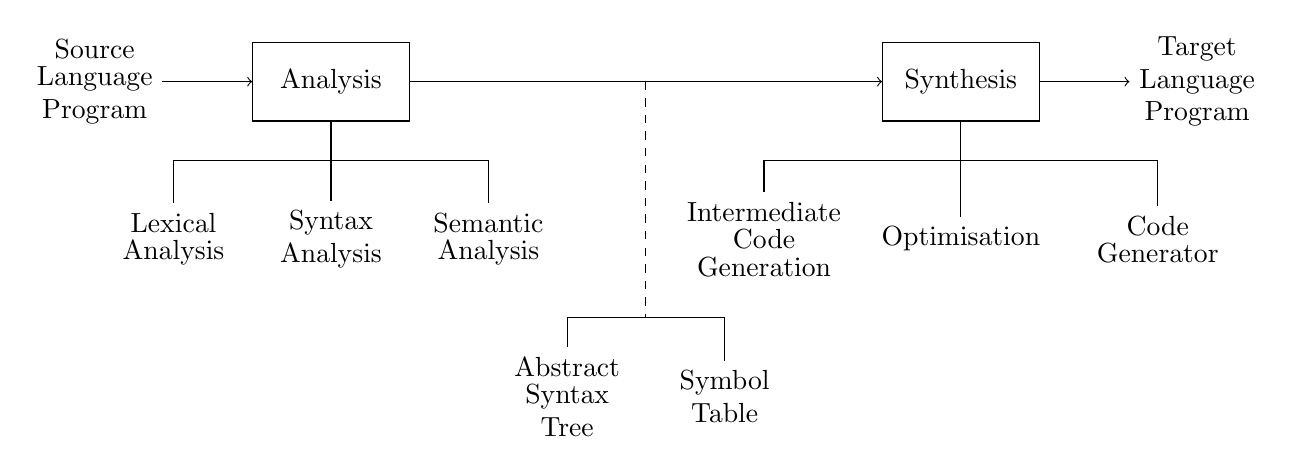
\begin{tikzpicture}
                        \node (slp) at (0, 0) {\shortstack{Source \\ Language \\ Program}};
                        \node (a) at (3, 0) {Analysis};
                        \node (s) at (11, 0) {Synthesis};
                        \node (tlp) at (14, 0) {\shortstack{Target \\ Language \\ Program}};

                        \node (la) at (1, -2) {\shortstack{Lexical \\ Analysis}};
                        \node (sa1) at (3, -2) {\shortstack{Syntax \\ Analysis}};
                        \node (sa2) at (5, -2) {\shortstack{Semantic \\ Analysis}};

                        \node (icg) at (8.5, -2) {\shortstack{Intermediate \\ Code \\ Generation}};
                        \node (o) at (11, -2) {Optimisation};
                        \node (cg) at (13.5, -2) {\shortstack{Code \\ Generator}};

                        \node (ast) at (6, -4) {\shortstack{Abstract \\ Syntax \\ Tree}};
                        \node (st) at (8, -4) {\shortstack{Symbol \\ Table}};

                        \draw
                        (slp) edge[->] (2, 0)
                        (4, 0) edge[->] (10, 0)
                        (12, 0) edge[->] (tlp)

                        (3, -0.5) -- (3, -1)
                        (11, -0.5) -- (11, -1)
                        (7, 0) edge[dashed] (7, -3)

                        (1, -1) -- (5, -1)
                        (1, -1) -- (la)
                        (3, -1) -- (sa1)
                        (5, -1) -- (sa2)

                        (8.5, -1) -- (13.5, -1)
                        (8.5, -1) -- (icg)
                        (11, -1) -- (o)
                        (13.5, -1) -- (cg)

                        (6, -3) -- (8, -3)
                        (6, -3) -- (ast)
                        (8, -3) -- (st)

                        (2, 0.5) -- (4, 0.5) -- (4, -0.5) -- (2, -0.5) -- cycle
                        (10, 0.5) -- (12, 0.5) -- (12, -0.5) -- (10, -0.5) -- cycle;
                    \end{tikzpicture}
                \end{center}
                \begin{itemize}
                    \itemsep0em
                    \item \textbf{lexical analysis} looks at characters of input program, analyses which are keywords (such as converting ~if~, and ~while~ to corresponding tokens), which are user defined words, and which are punctuation, etc.
                    \item \textbf{syntax analysis} discovers structure of input
                    \item \textbf{semantic analysis} checks that variables are declared before they are used, and that they are used consistently with their types etc.
                \end{itemize}
                Simple compilers go straight to code generation, but optimising compilers do several passes of intermediate code generation and optimisation.
                \smallskip

                The symbol table holds data on variables, such as types.
                Sometimes we need to know the type of the variable, in order to generate code for the variable, for example if we were to print a variable, it would need to generate different code for strings than it would need to do for integers.
                Scope rules are also needed.
            \subsubsection*{Phases}
                Whether all of these phases are done in the order shown is a design choice.
                For example, lexical analysis and syntax analysis are often interleaved.
                This can be done when the syntax analysis stage needs the next symbol, and therefore the lexical analysis stage can be used.
                \begin{center}
                    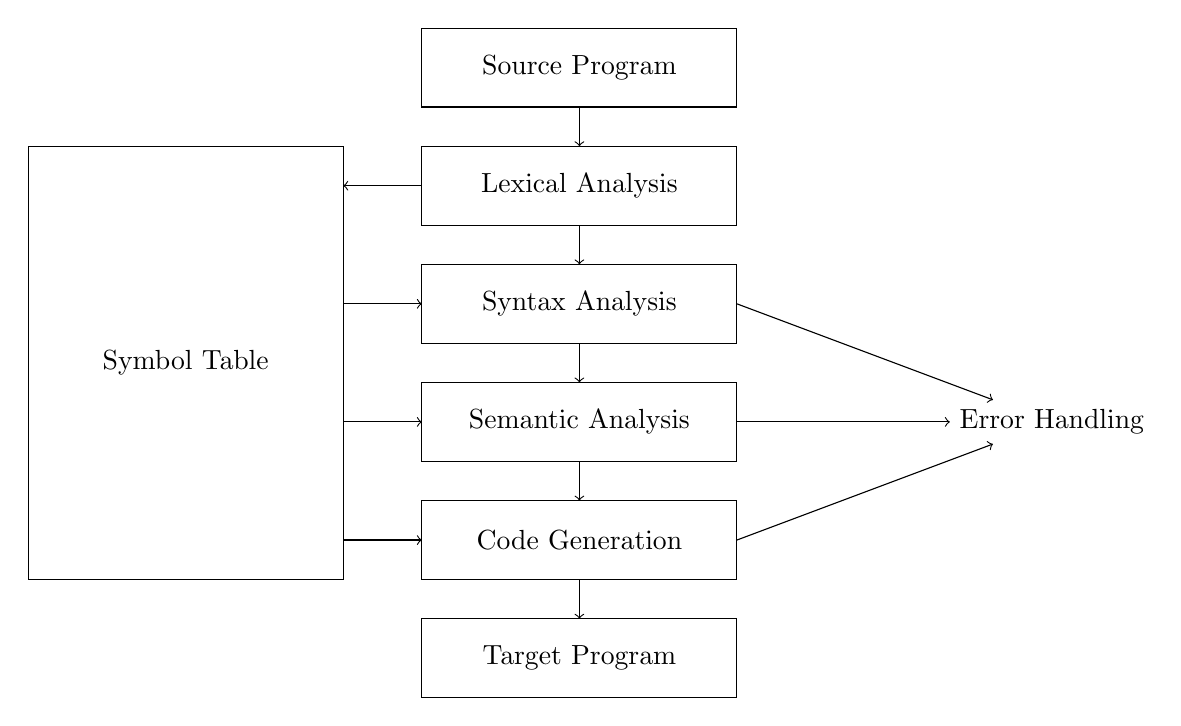
\begin{tikzpicture}
                        \node () at (0, 0) {Source Program};
                        \node () at (0, -1.5) {Lexical Analysis};
                        \node () at (0, -3) {Syntax Analysis};
                        \node () at (0, -4.5) {Semantic Analysis};
                        \node () at (0, -6) {Code Generation};
                        \node () at (0, -7.5) {Target Program};
                        \node () at (-5, -3.75) {Symbol Table};
                        \node (eh) at (6, -4.5) {Error Handling};

                        \draw
                        (-2, 0.5) -- (2, 0.5) -- (2, -0.5) -- (-2, -0.5) -- cycle
                        (-2, -1) -- (2, -1) -- (2, -2) -- (-2, -2) -- cycle
                        (-2, -2.5) -- (2, -2.5) -- (2, -3.5) -- (-2, -3.5) -- cycle
                        (-2, -4) -- (2, -4) -- (2, -5) -- (-2, -5) -- cycle
                        (-2, -5.5) -- (2, -5.5) -- (2, -6.5) -- (-2, -6.5) -- cycle
                        (-2, -7) -- (2, -7) -- (2, -8) -- (-2, -8) -- cycle
                        (-7, -1) -- (-3, -1) -- (-3, -6.5) -- (-7, -6.5) -- cycle

                        (0, -0.5) edge[->] (0, -1)
                        (0, -2) edge[->] (0, -2.5)
                        (0, -3.5) edge[->] (0, -4)
                        (0, -5) edge[->] (0, -5.5)
                        (0, -6.5) edge[->] (0, -7)
                        (-2, -1.5) edge[->] (-3, -1.5)
                        (-3, -3) edge[->] (-2, -3)
                        (2, -3) edge[->] (eh)
                        (-3, -4.5) edge[->] (-2, -4.5)
                        (2, -4.5) edge[->] (eh)
                        (-3, -6) edge[->] (-2, -6)
                        (2, -6) edge[->] (eh);
                    \end{tikzpicture}
                \end{center}
            \subsubsection*{Syntax Analysis}
                This is also known as parsing.
                Languages have a grammatical structure specified by grammatical rules in a \textbf{context-free grammar} such as BNF (\textbf{Backus-Naur Form}).
                The output of the analyser is a data structure which represents the program structure; an \textbf{abstract syntax tree}.
                The writer of the compiler must design the AST carefully such that it is easy to build, as well as easy to use by the code generator.
                \smallskip

                A language specification consists of the following;
                \begin{itemize}
                    \itemsep0em
                    \item \textbf{syntax} \hfill grammatical structure
                        \subitem in order to determine that a program is syntactically correct, one must determine how the rules were used to construct it
                    \item \textbf{semantics} \hfill meaning
                \end{itemize}
                For example, we can encode the rules for a statement as follows (anything in quotes is a terminal), in BNF;
                \begin{center}
                    stat $\to$ 'if' '(' exp ')' stat 'else' stat
                \end{center}
                Each BNF production is a valid way for a non-terminal (LHS) to be expanded (RHS) into a combination of terminals and non-terminals.
                Only terminals can appear in the final results (they are lexical tokens).
                \smallskip

                To prove the following is a valid example of stat, we'd need to show that a can be derived from exp, and that both b and c can be derived from stat.
                \begin{center}
                    if ( a ) b else c
                \end{center}
            \subsubsection*{Context-Free Grammars}
                Formally, a context-free grammar consists of the following four components;
                \begin{itemize}
                    \itemsep0em
                    \item $S$ \hfill a non-terminal start symbol
                    \item $P$ \hfill a set of productions
                    \item $t$ \hfill a set of tokens (terminals)
                    \item $nt$ \hfill a set of non-terminals
                \end{itemize}
                For example, consider the following BNF, and their associated components;
                \begin{align*}
                    \text{bin} \to &\ \text{bin '+' dig} \bnfsep \text{bin '-' dig} \bnfsep \text{dig} \\
                    \text{dig} \to &\ \text{'0'} \bnfsep \text{'1'} \\
                    t = &\ \{ \text{'+'}, \text{'-'}, \text{'0'}, \text{'1'}\} \\
                    nt = &\ \{ \text{bin}, \text{dig}\} \\
                    S = &\ \text{bin}
                \end{align*}
                A string of only terminals (\textbf{sentential form}) can be derived using the grammar by beginning with the start symbol, and repeatedly replacing each non-terminal with the RHS from a corresponding production.
                We refer to the set of all sentential forms derived from the start symbol as the \textbf{language} of a grammar.
                \smallskip

                We can prove that some string is in the language of a grammar by constructing a \textbf{parse tree}.
                For example, to prove that $\text{"1+1-0"} \in L(G)$, and $\text{"1+1"} \in L(G)$ we can use the following trees;
                \begin{center}
                    \begin{tikzpicture}[x=2cm]
                        \node (b1) at (0, 0) {bin};
                        \node (b2) at (-1, -1) {bin};
                        \node (b3) at (-2, -2) {bin};
                        \node (d1) at (1, -1) {dig};
                        \node (d2) at (0, -2) {dig};
                        \node (d3) at (-2, -3) {dig};
                        \node (o1) at (-2, -4) {'1'};
                        \node (o2) at (0, -3) {'1'};
                        \node (z) at (1, -2) {'0'};
                        \node (m) at (0, -1) {'-'};
                        \node (p) at (-1, -2) {'+'};

                        \draw
                        (b1) -- (d1) -- (z)
                        (b1) -- (m)
                        (b2) -- (d2) -- (o2)
                        (b2) -- (p)
                        (b1) -- (b2) -- (b3) -- (d3) -- (o1);
                    \end{tikzpicture}
                    \hfill
                    \begin{tikzpicture}[x=2cm]
                        \node (b1) at (0, 0) {bin};
                        \node (b2) at (-1, -1) {bin};
                        \node (d1) at (1, -1) {dig};
                        \node (d2) at (-1, -2) {dig};
                        \node (o1) at (-1, -3) {'1'};
                        \node (o2) at (1, -2) {'1'};
                        \node (p) at (0, -1) {'+'};

                        \draw
                        (b1) -- (d1) -- (o2)
                        (b1) -- (p)
                        (b1) -- (b2) -- (d2) -- (o1);
                    \end{tikzpicture}
                \end{center}
            \subsubsection*{Ambiguity}
                A grammar is referred to as \textbf{ambiguous} if its language contains strings which can be generated in two different ways.
                Essentially, there exists some string in $L(G)$ which has two different parse trees.
                Consider string "1 + a - 3" in the following grammar, and the parse tree(s) associated;
                \begin{center}
                    exp $\to$ exp '+' exp \vline\ exp '-' exp \vline\ const \vline\ ident
                \end{center}
                \begin{center}
                    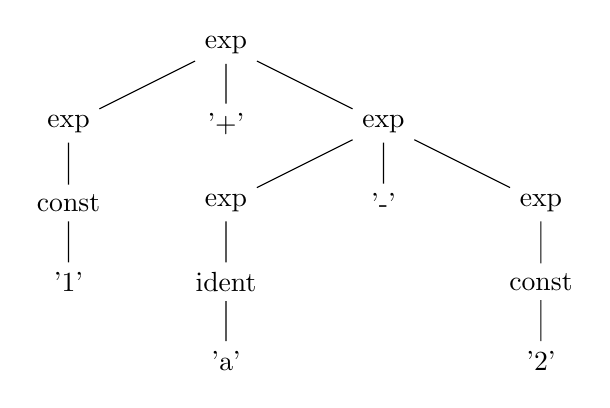
\begin{tikzpicture}[x=2cm]
                        \node (e1) at (0, 0) {exp};
                        \node (e2) at (-1, -1) {exp};
                        \node (e3) at (1, -1) {exp};
                        \node (e4) at (0, -2) {exp};
                        \node (e5) at (2, -2) {exp};
                        \node (c1) at (-1, -2) {const};
                        \node (c2) at (2, -3) {const};
                        \node (i) at (0, -3) {ident};
                        \node (p) at (0, -1) {'+'};
                        \node (m) at (1, -2) {'-'};
                        \node (o) at (-1, -3) {'1'};
                        \node (a) at (0, -4) {'a'};
                        \node (t) at (2, -4) {'2'};
                        \draw
                        (e1) -- (e2) -- (c1) -- (o)
                        (e1) -- (p)
                        (e1) -- (e3) -- (e4) -- (i) -- (a)
                        (e3) -- (m)
                        (e3) -- (e5) -- (c2) -- (t);
                    \end{tikzpicture}
                    \hfill
                    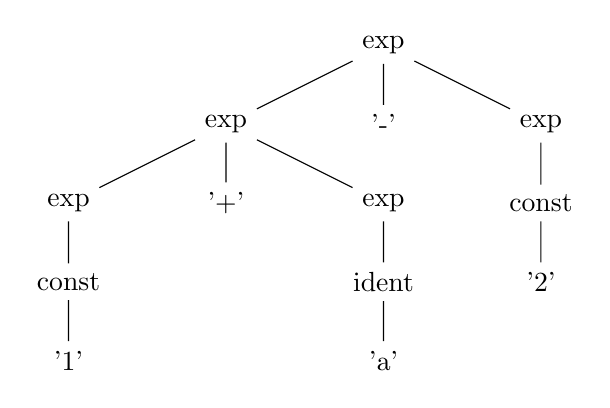
\begin{tikzpicture}[x=2cm]
                        \node (e1) at (0, 0) {exp};
                        \node (e2) at (-1, -1) {exp};
                        \node (e3) at (1, -1) {exp};
                        \node (e4) at (-2, -2) {exp};
                        \node (e5) at (0, -2) {exp};
                        \node (c1) at (1, -2) {const};
                        \node (c2) at (-2, -3) {const};
                        \node (i) at (0, -3) {ident};
                        \node (p) at (-1, -2) {'+'};
                        \node (m) at (0, -1) {'-'};
                        \node (o) at (-2, -4) {'1'};
                        \node (a) at (0, -4) {'a'};
                        \node (t) at (1, -3) {'2'};
                        \draw
                        (e1) -- (e2) -- (e4) -- (c2) -- (o)
                        (e1) -- (m)
                        (e1) -- (e3) -- (c1) -- (t)
                        (e2) -- (p)
                        (e2) -- (e5) -- (i) -- (a);
                    \end{tikzpicture}
                \end{center}
                While the string is still valid, and in the language, our issue is with the ambiguity, as we want to generate a program uniquely.
                The reason our grammar is broken is due to the recursive use of the non-terminal exp on both sides, which means we're given a choice of which side to expand when generating.
            \subsubsection*{Associativity and Precedence}
                For our example language, we're using all left-associative operators.
                We also want to maintain that '*' and '/' have higher precedence than '+' and '-'.
                One way of doing this is to split the grammar into layers, by having separate non-terminals for precedence levels.
                This method can be done with the following unambiguous grammar for arithmetic expressions;
                \begin{align*}
                    \text{exp} & \to \text{exp '+' term} \bnfsep \text{exp '-' term} \bnfsep \text{term} \\
                    \text{term} & \to \text{term '*' factor} \bnfsep \text{term '/' factor} \bnfsep \text{factor} \\
                    \text{factor} & \to \text{const} \bnfsep \text{ident}
                \end{align*}
                Now, we can unambiguously generate the parse tree (and thus the unique abstract syntax tree) for "9+5*2";
                \begin{center}
                    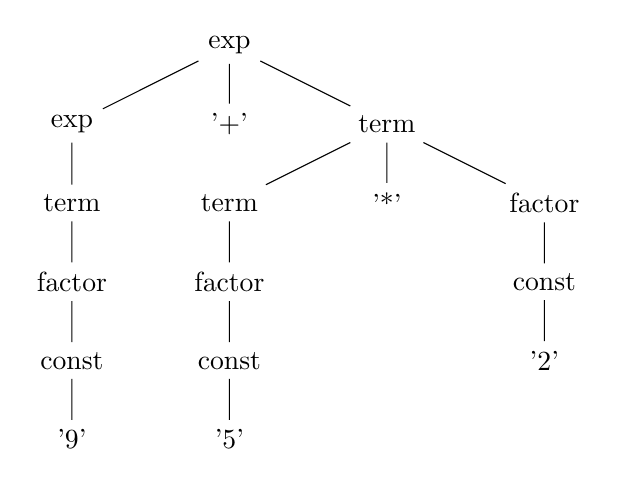
\begin{tikzpicture}[x=2cm]
                        \node (e1) at (0, 0) {exp};
                        \node (e2) at (-1, -1) {exp};
                        \node (t1) at (1, -1) {term};
                        \node (t2) at (-1, -2) {term};
                        \node (t3) at (0, -2) {term};
                        \node (f1) at (2, -2) {factor};
                        \node (f2) at (-1, -3) {factor};
                        \node (f3) at (0, -3) {factor};
                        \node (c1) at (2, -3) {const};
                        \node (c2) at (-1, -4) {const};
                        \node (c3) at (0, -4) {const};
                        \node (p) at (0, -1) {'+'};
                        \node (m) at (1, -2) {'*'};
                        \node (n) at (-1, -5) {'9'};
                        \node (f) at (0, -5) {'5'};
                        \node (t) at (2, -4) {'2'};
                        \draw
                        (e1) -- (e2) -- (t2) -- (f2) -- (c2) -- (n)
                        (e1) -- (p)
                        (e1) -- (t1) -- (t3) -- (f3) -- (c3) -- (f)
                        (t1) -- (m)
                        (t1) -- (f1) -- (c1) -- (t);
                    \end{tikzpicture}
                    \hfill
                    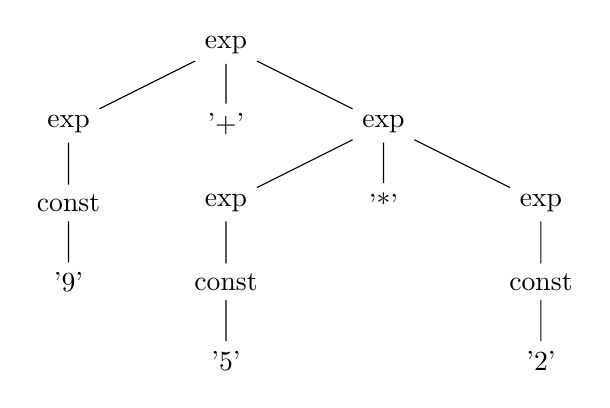
\begin{tikzpicture}[x=2cm]
                        \node (e1) at (0, 0) {exp};
                        \node (e2) at (-1, -1) {exp};
                        \node (p) at (0, -1) {'+'};
                        \node (e3) at (1, -1) {exp};
                        \node (c1) at (-1, -2) {const};
                        \node (e4) at (0, -2) {exp};
                        \node (m) at (1, -2) {'*'};
                        \node (e5) at (2, -2) {exp};
                        \node (n) at (-1, -3) {'9'};
                        \node (c2) at (0, -3) {const};
                        \node (c3) at (2, -3) {const};
                        \node (f) at (0, -4) {'5'};
                        \node (t) at (2, -4) {'2'};
                        \draw
                        (e1) -- (e2) -- (c1) -- (n)
                        (e1) -- (p)
                        (e1) -- (e3) -- (e4) -- (c2) -- (f)
                        (e3) -- (m)
                        (e3) -- (e5) -- (c3) -- (t);
                    \end{tikzpicture}
                \end{center}
                It's important to note that the \textbf{abstract} syntax tree doesn't need this in contrast, as only the parse tree needs it.
            \subsubsection*{Parsers}
                The parser checks that the input is grammatically correct, and builds an AST representing the structure.
                In general, there are two classes of parsing algorithms;
                \begin{itemize}
                    \itemsep0em
                    \item \textbf{top-down / predictive} \hfill we are using recursive descent
                    \item \textbf{bottom-up} \hfill also known as shift-reduce
                \end{itemize}
                For this, we will use the input "~begin S; S; end~", with the following grammar;
                \begin{align*}
                    \text{stat} & \to ~'begin'~\ \text{statlist} \bnfsep ~'S'~ \\
                    \text{statlist} & \to ~'end'~ \bnfsep \text{stat}\ ~';'~\ \text{statlist}
                \end{align*}
                When we start top-down parsing, we start with the non-terminal stat.
                The first token we identify is the ~'begin'~, thus our tree becomes the following;
                \begin{center}
                    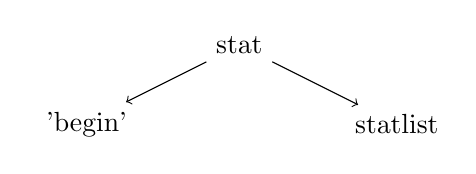
\begin{tikzpicture}[x=2cm]
                        \node (s) at (0, 0) {stat};
                        \node (b) at (-1, -1) {~'begin'~};
                        \node (sl) at (1, -1) {statlist};

                        \draw
                        (s) edge[->] (b)
                        (s) edge[->] (sl);
                    \end{tikzpicture}
                \end{center}
                However, as the next symbol isn't the terminal ~'end'~, we have to use an alternative.
                As we only have one alternative, we can predict it, and thus the tree becomes;
                \begin{center}
                    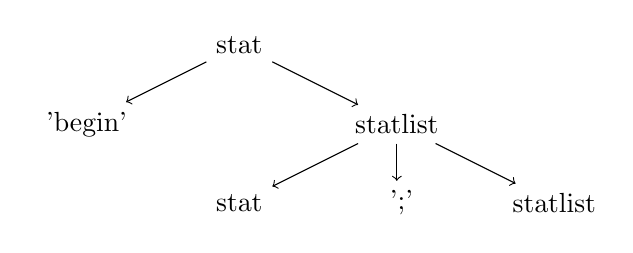
\begin{tikzpicture}[x=2cm]
                        \node (s) at (0, 0) {stat};
                        \node (b) at (-1, -1) {~'begin'~};
                        \node (sl) at (1, -1) {statlist};
                        \node (s2) at (0, -2) {stat};
                        \node (sc) at (1, -2) {~';'~};
                        \node (sl2) at (2, -2) {statlist};

                        \draw
                        (s) edge[->] (b)
                        (s) edge[->] (sl)
                        (sl) edge[->] (s2)
                        (sl) edge[->] (sc)
                        (sl) edge[->] (sl2);
                    \end{tikzpicture}
                \end{center}
                As the next symbols are the terminal ~'S'~, and the terminal ~';'~, we can tick them off, thus the tree becomes;
                \begin{center}
                    \begin{tikzpicture}[x=2cm]
                        \node (s) at (0, 0) {stat};
                        \node (b) at (-1, -1) {~'begin'~};
                        \node (sl) at (1, -1) {statlist};
                        \node (s2) at (0, -2) {stat};
                        \node (sc) at (1, -2) {~';'~};
                        \node (sl2) at (2, -2) {statlist};
                        \node (st) at (0, -3) {~'S'~};

                        \draw
                        (s) edge[->] (b)
                        (s) edge[->] (sl)
                        (sl) edge[->] (s2)
                        (sl) edge[->] (sc)
                        (sl) edge[->] (sl2)
                        (s2) edge[->] (st);
                    \end{tikzpicture}
                \end{center}
                This process continues, until we reach the final tree;
                \begin{center}
                    \begin{tikzpicture}[x=2cm]
                        \node (s) at (0, 0) {stat};
                        \node (b) at (-1, -1) {~'begin'~};
                        \node (sl) at (1, -1) {statlist};
                        \node (s2) at (0, -2) {stat};
                        \node (sc) at (1, -2) {~';'~};
                        \node (sl2) at (2, -2) {statlist};
                        \node (st) at (0, -3) {~'S'~};
                        \node (s3) at (1, -3) {stat};
                        \node (sc2) at (2, -3) {~';'~};
                        \node (sl3) at (3, -3) {statlist};
                        \node (st2) at (1, -4) {~'S'~};
                        \node (e) at (3, -4) {~'end'~};

                        \draw
                        (s) edge[->] (b)
                        (s) edge[->] (sl)
                        (sl) edge[->] (s2)
                        (sl) edge[->] (sc)
                        (sl) edge[->] (sl2)
                        (s2) edge[->] (st)
                        (sl2) edge[->] (s3)
                        (sl2) edge[->] (sc2)
                        (sl2) edge[->] (sl3)
                        (s3) edge[->] (st2)
                        (sl3) edge[->] (e);
                    \end{tikzpicture}
                \end{center}
                On the other hand, bottom-up parsing tries to use all the RHSs (whereas top-down tries to match a non-terminal by trying each of the RHSs), and replaces it with a non-terminal, by using the production in reverse.
                Bottom-up succeeds when the whole input is replaced by the start symbol.
                \smallskip

                In general, we push the current symbol onto the stack (or the reduction if we can reduce it).
                For example, once we encounter ~'S'~, we can reduce it to stat, and similarly once we encounter ~'end'~, we can reduce it to statlist.
                \begin{center}
                    \begin{tabular}{|r|c|l|l|l|}
                        \hline
                        stack & current symbol & remaining tokens & S/R & note \\
                        \hline
                        & ~'begin'~ & ~'S'~ ~';'~ ~'S'~ ~';'~ ~'end'~ & S & nothing to do yet \\
                        ~'begin'~ & \violet{~'S'~} & ~';'~ ~'S'~ ~';'~ ~'end'~ & R & terminal for stat \\
                        ~'begin'~ & \blue{stat} & ~';'~ ~'S'~ ~';'~ ~'end'~ & S & no more work \\
                        ~'begin'~ \blue{stat} & ~';'~ & ~'S'~ ~';'~ ~'end'~ & S & nothing to do yet \\
                        ~'begin'~ \blue{stat} ~';'~ & \violet{~'S'~} & ~';'~ ~'end'~ & R & terminal for stat \\
                        ~'begin'~ stat ~';'~ & \blue{stat} & ~';'~ ~'end'~ & S & no more work \\
                        ~'begin'~ stat ~';'~ \blue{stat} & ~';'~ & ~'end'~ & S & nothing to do yet \\
                        ~'begin'~ stat ~';'~ stat ~';'~ & \violet{~'end'~} & & R & terminal for statlist \\
                        ~'begin'~ stat ~';'~ stat ~';'~ & \blue{statlist} & & & \\
                        ~'begin'~ stat ~';'~ \violet{stat} \violet{~';'~} & \violet{statlist} & & R & match for statlist \\
                        ~'begin'~ stat ~';'~ & \blue{statlist} & & & \\
                        ~'begin'~ \violet{stat} \violet{~';'~} & \violet{statlist} & & R & match for statlist \\
                        ~'begin'~ & \blue{statlist} & & & \\
                        \violet{~'begin'~} & \violet{statlist} & & R & match for stat \\
                        & \blue{stat} & & & complete \\
                        \hline
                    \end{tabular}
                \end{center}
            \subsubsection*{Simple Compiler in Haskell}
                If the input to the parser is a simple string of characters, representing an arithmetic expression, following the BNF defined below;
                \begin{align*}
                    \text{expr} & \to \text{fact '+' expr} \bnfsep \text{fact} \\
                    \text{fact} & \to \text{number} \bnfsep \text{identifier}
                \end{align*}
                The string ~a + b + 1~ would become the following sequence of tokens, after lexical analysis;
                \begin{center}
                    ~[IDENT "a", PLUS, IDENT "b", PLUS, NUM 1]~
                \end{center}
                It's important to note that this is a right-recursive grammar, as a recursive descent method \textbf{will not} work with left-recursive grammars.
                \begin{lstlisting}
                    data Token
                      = IDENT [Char] | NUM Int | PLUS
                    data Ast
                      = Ident [Char] | Num Int | Plus Ast Ast
                      deriving (Show)
                    data Instr
                      = PushVar [Char] | PushConst Int | Add
                      deriving (Show)
                    parse :: [Token] -> Ast
                    parse ts =
                      let (tree, ts') = parseExpr ts
                      in case ts' of
                        [] -> tree
                        _  -> error "Excess tokens"
                    parseExpr :: [Token] -> (Ast, [Token])
                    parseExpr ts
                      = let (factTree, ts') = parseFact ts
                        in case ts' of
                          (PLUS : ts') ->
                            let (sExpTree, ts'') = parseExpr ts'
                            in (Plus factTree sExpTree, ts'')
                          other -> (factTree, other)
                    parseFact :: [Token] -> (Ast, [Token])
                    parseFact (t:ts)
                      = case t of
                          NUM n -> (Num n, ts)
                          IDENT x -> (Ident x, ts)
                          _ -> error "Expected a number or identifier"
                    translate :: Ast -> [Instr]
                    translate ast
                      = case ast of
                          Num n -> PushConst n
                          Ident x -> PushVar x
                          Plus e1 e2 -> translate e1 ++ translate e2 ++ [Add]
                \end{lstlisting}
                Comments on the code;
                \begin{itemize}
                    \itemsep0em
                    \item Note that the structures for ~Token~ and ~Ast~, defined on lines 2 and 4 respectively, are very similar - however, the latter represents a tree structure
                    \item We require a parsing function for each non-terminal in the code, hence we have ~parseExpr~ and ~parseFact~
                    \item It's easier to start with the non-recursive cases, which are the factors
                    \item From here, you can see that the recursion structure of the code closely follows the recursion structure of the grammar, as we have the recursion in line 20 (on expressions, after the factor is parsed)
                    \item Each function returns the part of the AST it has generated and the \textbf{remaining} tokens after consuming input
                    \item The final translation function generates instructions for a very simple stack machine
                \end{itemize}
        \subsection*{13th January 2020}
            \subsubsection*{Bootstrapping}
                Imagine the scenario where there is a new language, and only one machine.
                The process of writing a compiler for this language, with this language, is to first manually write a compiler in the assembly language for the machine for a small subset of the new language.
                Using the subset of this new language (that can be compiled), we can write a compiler to compile more of the language, and this process continues until we can compile the entire language.
            \subsubsection*{Lexical Analysis}
                The lexical analyser (sometimes called a scanner) converts characters into tokens.
                This is because the compiler shouldn't have to deal with strings directly.
                Normally, this removes whitespace, as it isn't needed in code generation (other than for string / character literals).
                In this course, the regular expressions that the scanners use will be converted into finite automata.
                \medskip

                Identifiers are usually classified into the following;
                \begin{itemize}
                    \itemsep0em
                    \item \textbf{keywords}
                        \medskip

                        These are defined by the language, and are reserved.
                        For example, words such as "return", "for", "class", and so on are represented as their own tokens (~RETURN~, ~FOR~, and ~CLASS~ respectively), since there is a (relatively) small finite set to work with.
                        The scanner needs to be able to quickly verify if something is a keyword, and therefore something such as a "perfect" hash function is used.
                    \item \textbf{user-defined}
                        \medskip

                        These are defined by the programmer.
                        Since there can be (theoretically) an infinite amount of them, it's not possible to generate a unique token for each one, and therefore it usually falls under a general identifier token with a string parameter (such that "xyz" becomes ~IDENT("xyz")~, or similar).
                \end{itemize}
                In the case of literals, some special consideration may be needed for cases where the language we are compiling can support more than the language we are writing the compiler in.
                For example, if the language we are writing a compiler for can support arbitrarily large integers, special consideration will be required if the language the compiler is written in cannot support such values.
                Some examples of literals are as follows (more can exist, such as booleans, characters, and so on);
                \begin{itemize}
                    \itemsep0em
                    \item \textbf{integers}
                        \medskip

                        An integer would likely be represented by a general integer token, such that the string "123" would become ~INTEGER(123)~, or similar.
                    \item \textbf{strings}
                        \medskip

                        Similar to integers, but the token constructor will now take a string parameter instead of an integer, such that ""foo"" would become ~STRING("foo")~.
                \end{itemize}
                There are other tokens, not just the two cases above, such as (but not limited to);
                \begin{itemize}
                    \itemsep0em
                    \item \textbf{operators / symbols}
                        \medskip

                        Normally operators / symbols such as "+", "<=", "(" are represented as their own unique token, such as ~PLUS~, ~LTE~, ~LPAREN~, respectively.
                    \item \textbf{whitespace / comments}
                        \medskip

                        Whitespace characters are normally removed (unless they are in the case where they exist within a literal), but are needed to separate adjacent identifiers.
                        Comments are also usually removed.
                \end{itemize}
            \subsubsection*{Regular Expressions (Regex)}
                This allows us to formally define the acceptable tokens of the language.
                \begin{center}
                    \begin{tabular}{ll}
                        regex & matches \\
                        \hline
                        ~a~ & a literal \textbf{symbol} of the language's alphabet (that isn't a regex meta-character) \\
                        $\epsilon$ & the empty string \textbf{epsilon} \\
                        ~R1 R2~ & \textbf{concatenation} of regex ~R1~ followed by ~R2~ (medium precedence) \\
                        ~R1|R2~ & \textbf{alternation} of regex ~R1~ or ~R2~ (lowest precedence) \\
                        ~R*~ & \textbf{repetition} of regex ~R~ (0 or more times) (highest precedence) \\
                        ~(R)~ & \textbf{grouping} ~R~ by itself, used to override precedence \\
                        ~\ttbs{}a~ & "escaping", used to have a literal of a meta-character \\
                        \hline
                        shortcut & (can be made by the rules above) \\
                        \hline
                        ~R?~ & 0 or 1 occurrences of regex ~R~ \\
                        ~R+~ & 1 or more occurrences of regex ~R~ \\
                        ~[aeiou123]~ & any character from the given set \\
                        ~[a-zA-Z0-9]~ & any alphanumeric character \\
                        ~[\^{}a-zA-Z]~ & any character \textbf{except} the ones in the set \\
                        ~.~ & any character except a newline
                    \end{tabular}
                \end{center}
        \subsection*{15th January 2020}
            \subsubsection*{Regular Expression Rules}
                We write rules or productions in the form $\alpha \to ~X~$, where $\alpha$ is a non-terminal (the name of the rule), and ~X~ is some regular expressions constructed by any combination of terminals (symbols) and non-terminals (names of \textbf{other} rules - recursion is not allowed, therefore all non-terminals must be defined before being used in another rule).
                For example, we have the following regular expressions for a simple grammar (note that it looks very similar to WACC).
                \begin{align*}
                    \underline{~Digit~} & \to ~[0-9]~ \\
                    \underline{~Int~} & \to \underline{~Digit~}~+~ \\
                    \underline{~SignedDigit~} & \to ~(+ | -)? \underline{~Int~}~ \\
                    \underline{~Keyword~} & \to ~if | while | do~ \\
                    \underline{~Identifier~} & \to ~\underline{~Letter~} (\underline{~Letter~} | \underline{~Digit~})*~
                \end{align*}
                However, we can run into the issue of ambiguity, when a character sequence can match to more than one regex.
                For example, the input string ~dough~ matches to the identifier ~dough~, as well as partially to the keyword ~do~.
                Two strategies are either to match the longest character sequence (causing the former), or to have textual precedence, where the first regex takes precedence (causing the latter).
            \subsubsection*{Finite Automata}
                When we draw a finite automata, its important to note the following symbols we use;
                \begin{itemize}
                    \itemsep0em
                    \item \textbf{states} are circles
                        \begin{itemize}
                            \itemsep0em
                            \item the \textbf{start} state has an unlabelled arrow going into it
                            \item the \textbf{accepting} (end) state is a double circle
                            \item all non-accepting states have arrows leading to an error state, but this is often omitted
                        \end{itemize}
                    \item \textbf{transitions} are arrows between states, with the matched \textbf{symbol} being the labels of the arrows
                \end{itemize}
                The types of finite automata we look at are the following;
                \begin{itemize}
                    \itemsep0em
                    \item \textbf{deterministic finite automata (DFA)}
                        \begin{center}
                            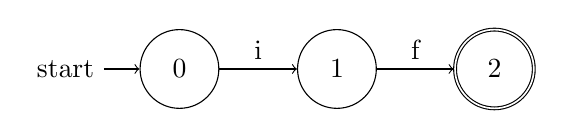
\begin{tikzpicture}
                                \node[state, minimum size=1cm, initial] (0) at (0, 0) {$0$};
                                \node[state, minimum size=1cm] (1) at (2, 0) {$1$};
                                \node[state, minimum size=1cm, accepting] (2) at (4, 0) {$2$};

                                \draw
                                (0) edge[->, above] node{i} (1)
                                (1) edge[->, above] node{f} (2);
                            \end{tikzpicture}
                        \end{center}
                        The example above is deterministic as there are no two transitions from the same state with the same symbol.
                    \item \textbf{non-deterministic finite automata (NFA)}
                        \begin{center}
                            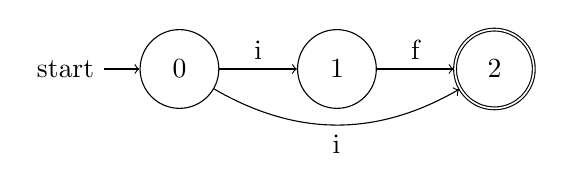
\begin{tikzpicture}
                                \node[state, minimum size=1cm, initial] (0) at (0, 0) {$0$};
                                \node[state, minimum size=1cm] (1) at (2, 0) {$1$};
                                \node[state, minimum size=1cm, accepting] (2) at (4, 0) {$2$};

                                \draw
                                (0) edge[->, above] node{i} (1)
                                (0) edge[->, bend right=30, below] node{i} (2)
                                (1) edge[->, above] node{f} (2);
                            \end{tikzpicture}
                        \end{center}
                        The example above is non-deterministic as there is more than one transition from state 0 with the same symbol.
                        It allows for choice and more compact solutions, but requires backtracking.
                \end{itemize}
            \subsubsection*{Conversion of Regex to (Non-Deterministic) Finite Automata}
                \textbf{Thompson's construction} uses $\epsilon$-transitions to "glue" together automata.
                While this is usually represented with an $\epsilon$ over the transition, it can be omitted for brevity, and therefore any transitions without labels will be assumed to be $\epsilon$-transitions.
                In lieu of repeatedly drawing the same thing, let the regular expression ~R1~ have an initial state of $p$ and an accepting / end state of $q$, and let ~R2~ have an initial state $r$ and accepting state $s$.
                Also note that within the dotted lines can exist an arbitrarily complex automata.
                \begin{center}
                    \begin{tabular}{>{\centering\arraybackslash}m{1.5cm}>{\centering\arraybackslash}m{10cm}}
                        regex & FA \\
                        \hline \\
                        ~a~ &
                        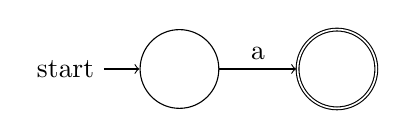
\begin{tikzpicture}
                            \node[state, minimum size=1cm, initial] (0) at (0, 0) {};
                            \node[state, minimum size=1cm, accepting] (1) at (2, 0) {};

                            \draw
                            (0) edge[->, above] node{a} (1);
                        \end{tikzpicture} \\
                        $\epsilon$ &
                        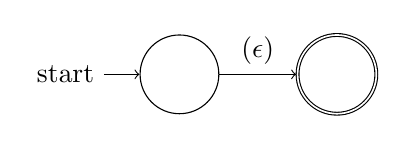
\begin{tikzpicture}
                            \node[state, minimum size=1cm, initial] (0) at (0, 0) {};
                            \node[state, minimum size=1cm, accepting] (1) at (2, 0) {};

                            \draw
                            (0) edge[->, above] node{$(\epsilon)$} (1);
                        \end{tikzpicture} \\
                        ~R1~ &
                        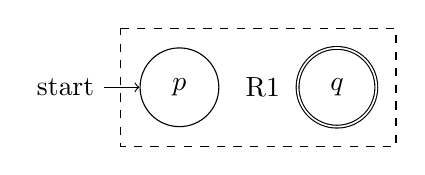
\begin{tikzpicture}
                            \node[state, minimum size=1cm, initial] (p) at (0, 0) {$p$};
                            \node[state, minimum size=1cm, accepting] (q) at (2, 0) {$q$};

                            \node at ($0.5*(p) + 0.5*(q)$) {~R1~};

                            \draw[dashed] ($(p) + (-0.75, 0.75)$) -- ($(q) + (0.75, 0.75)$) -- ($(q) + (0.75, -0.75)$) -- ($(p) + (-0.75, -0.75)$) -- cycle;
                        \end{tikzpicture} \\
                        ~R1 R2~ &
                        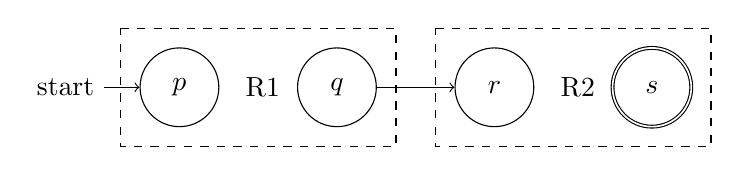
\begin{tikzpicture}
                            \node[state, minimum size=1cm, initial] (p) at (0, 0) {$p$};
                            \node[state, minimum size=1cm] (q) at (2, 0) {$q$};

                            \node at ($0.5*(p) + 0.5*(q)$) {~R1~};

                            \draw[dashed] ($(p) + (-0.75, 0.75)$) -- ($(q) + (0.75, 0.75)$) -- ($(q) + (0.75, -0.75)$) -- ($(p) + (-0.75, -0.75)$) -- cycle;

                            \node[state, minimum size=1cm] (r) at (4, 0) {$r$};
                            \node[state, minimum size=1cm, accepting] (s) at (6, 0) {$s$};

                            \node at ($0.5*(r) + 0.5*(s)$) {~R2~};

                            \draw[dashed] ($(r) + (-0.75, 0.75)$) -- ($(s) + (0.75, 0.75)$) -- ($(s) + (0.75, -0.75)$) -- ($(r) + (-0.75, -0.75)$) -- cycle;

                            \draw (q) edge[->] (r);
                        \end{tikzpicture} \\
                        ~R1|R2~ &
                        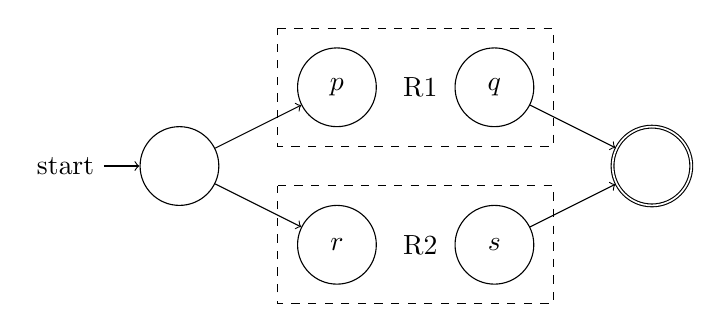
\begin{tikzpicture}
                            \node[state, minimum size=1cm, initial] (0) at (0, 0) {};
                            \node[state, minimum size=1cm, accepting] (1) at (6, 0) {};

                            \node[state, minimum size=1cm] (p) at (2, 1) {$p$};
                            \node[state, minimum size=1cm] (q) at (4, 1) {$q$};

                            \node at ($0.5*(p) + 0.5*(q)$) {~R1~};

                            \draw[dashed] ($(p) + (-0.75, 0.75)$) -- ($(q) + (0.75, 0.75)$) -- ($(q) + (0.75, -0.75)$) -- ($(p) + (-0.75, -0.75)$) -- cycle;

                            \node[state, minimum size=1cm] (r) at (2, -1) {$r$};
                            \node[state, minimum size=1cm] (s) at (4, -1) {$s$};

                            \node at ($0.5*(r) + 0.5*(s)$) {~R2~};

                            \draw[dashed] ($(r) + (-0.75, 0.75)$) -- ($(s) + (0.75, 0.75)$) -- ($(s) + (0.75, -0.75)$) -- ($(r) + (-0.75, -0.75)$) -- cycle;

                            \draw
                            (0) edge[->] (p)
                            (0) edge[->] (r)
                            (q) edge[->] (1)
                            (s) edge[->] (1);
                        \end{tikzpicture} \\
                        ~R1*~ &
                        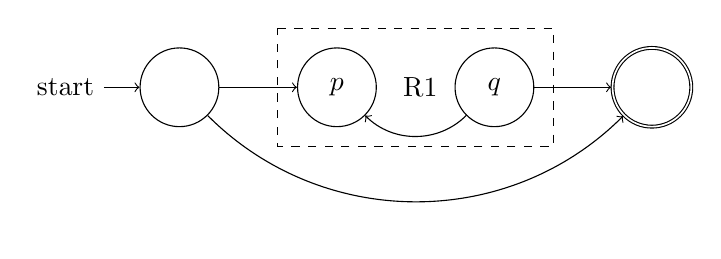
\begin{tikzpicture}
                            \node[state, minimum size=1cm, initial] (0) at (0, 0) {};
                            \node[state, minimum size=1cm, accepting] (1) at (6, 0) {};

                            \node[state, minimum size=1cm] (p) at (2, 0) {$p$};
                            \node[state, minimum size=1cm] (q) at (4, 0) {$q$};

                            \node at ($0.5*(p) + 0.5*(q)$) {~R1~};

                            \draw[dashed] ($(p) + (-0.75, 0.75)$) -- ($(q) + (0.75, 0.75)$) -- ($(q) + (0.75, -0.75)$) -- ($(p) + (-0.75, -0.75)$) -- cycle;

                            \draw
                            (0) edge[->] (p)
                            (0) edge[->, bend right=45] (1)
                            (q) edge[->] (1)
                            (q) edge[->, bend left=45] (p);
                        \end{tikzpicture} \\
                        \hline
                    \end{tabular}
                \end{center}
                For example, consider the regular expressions for an identifier, following the form ~L(L | D)*~, which represents a letter followed by any combination of letters and digits.
                Note that we are allowed to abbreviate the use of ~Letter~ to ~L~, for brevity, and similar for ~Digit~ to ~D~.
                \begin{center}
                    \begin{tikzpicture}
                        \node[state, minimum size=1cm, initial] (0) at (0, 0) {};
                        \node[state, minimum size=1cm] (1) at (2, 0) {};
                        \node[state, minimum size=1cm] (2) at (4, 0) {};
                        \node[state, minimum size=1cm] (3) at (10, 0) {};
                        \node[state, minimum size=1cm, accepting] (4) at (12, 0) {};
                        \node[state, minimum size=1cm] (l1) at (6, 1) {};
                        \node[state, minimum size=1cm] (l2) at (8, 1) {};
                        \node[state, minimum size=1cm] (d1) at (6, -1) {};
                        \node[state, minimum size=1cm] (d2) at (8, -1) {};

                        \draw
                        (0) edge[->, above] node{~L~} (1)
                        (1) edge[->] (2)
                        (1) edge[->, bend right=45] (4)
                        (2) edge[->] (l1)
                        (2) edge[->] (d1)
                        (l1) edge[->, above] node{~L~} (l2)
                        (d1) edge[->, above] node{~D~} (d2)
                        (l2) edge[->] (3)
                        (d2) edge[->] (3)
                        (3) edge[->] (4)
                        (3) edge[->, bend right=75] (2);
                    \end{tikzpicture}
                \end{center}
            \subsubsection*{Conversion from NFA to DFA}
                It's important to note the worst case complexities for NFA and DFA are as follows, where $n$ is the length of the input string, and $r$ is the length of the regular expression;
                \begin{center}
                    \begin{tabular}{l|c|c}
                        type & space complexity & time complexity \\
                        \hline
                        NFA & $O(r)$ & $O(nr)$ \\
                        DFA & $O(2^r)$ & $O(n)$
                    \end{tabular}
                \end{center}
                As you can see, DFAs are much faster, but can be exponentially bigger than NFAs.
                However, the worst case space complexity for a DFA is rarely reached for lexer analyser generators.
                \medskip

                In order to convert from NFA to DFA, we use $\epsilon$-closures.
                To avoid repetition, I will be denoting the $\epsilon$ closure of $s$ as $\epsilon_c(s)$.
                \begin{align*}
                    \epsilon_c(s) & = \text{set of states reachable by zero or more $\epsilon$-transitions from $s$} \\
                    \epsilon_c(\{s_1, \dots, s_n\}) & = \bigcup\limits_{i = 1}^{n} s_i
                \end{align*}
                For example, take the following NFA;
                \begin{center}
                    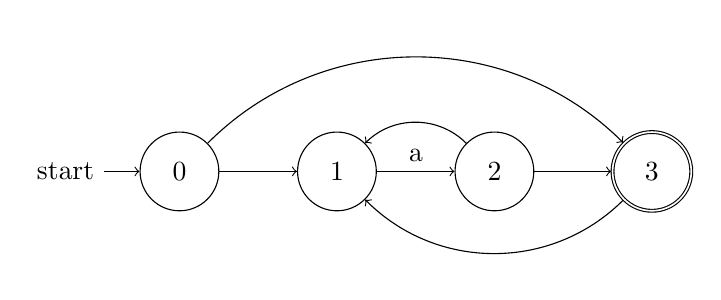
\begin{tikzpicture}
                        \node[state, minimum size=1cm, initial] (0) at (0, 0) {$0$};
                        \node[state, minimum size=1cm] (1) at (2, 0) {$1$};
                        \node[state, minimum size=1cm] (2) at (4, 0) {$2$};
                        \node[state, minimum size=1cm, accepting] (3) at (6, 0) {$3$};

                        \draw
                        (0) edge[->] (1)
                        (0) edge[->, bend left=45] (3)
                        (1) edge[->, above] node{a} (2)
                        (2) edge[->, bend right=45] (1)
                        (2) edge[->] (3)
                        (3) edge[->, bend left=45] (1);
                    \end{tikzpicture}
                \end{center}
                Which has the following closures;
                \begin{align*}
                    \epsilon_c(0) & = \{ 0, 1, 3 \} \\
                    \epsilon_c(1) & = \{ 1 \} \\
                    \epsilon_c(2) & = \{ 1, 2, 3 \} \\
                    \epsilon_c(3) & = \{ 1, 3 \}
                \end{align*}
                From our start state, using subset construction, we then create a node consisting of its $\epsilon$-closure.
                We look at this new node, find the ones that have a non-$\epsilon$-transition, and handle those cases.
                For each new case, we take the state that it goes to, and create a node consisting of its $\epsilon$-closure, and repeat the process.
                Finally, we mark each of the states that contain an accepting state as an accepting state.
                The example above becomes the following;
                \begin{center}
                    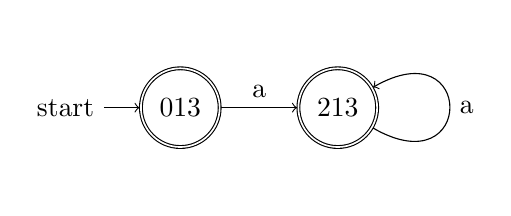
\begin{tikzpicture}
                        \node[state, minimum size=1cm, initial, accepting] (0) at (0, 0) {$013$};
                        \node[state, minimum size=1cm, accepting] (1) at (2, 0) {$213$};
                        \draw
                        (0) edge[->, above] node{a} (1)
                        (1) edge[->, loop, out=-30, in=30, right, distance=1.5cm] node{a} (1);
                    \end{tikzpicture}
                \end{center}
        \subsection*{17th January 2020}
            At the start of this lecture, he goes over the grammar for an example language that has statements, consisting of assignment and iteration.
            \subsubsection*{Code Generation for a Stack Machine}
                He then continues with a representation of a stack machine, it's a lot of reading, and most of it is on the slides.
                The general premise of the stack machine is that it fulfils a promise where it leaves the result of a computation at the top of the stack, and doesn't modify anything that was below it.
                As such, we end up with the following code (note that ~label1~ and ~label2~ are unique labels that haven't been used before - generating this in Haskell isn't as trivial as in other languages);
                \begin{lstlisting}
                    type Name = [Char]
                    type Label = [Char]

                    data Stat = Assign Name Exp | Seq Stat Stat | ForLoop Name Exp Exp Stat
                    data Exp = Binop Op Exp Exp | Unop Op Exp | Ident Name | Const Int
                    data Op = Plus | Minus | Times | Divide
                    data Instruction = Add | Sub | Mul | Div | Negate
                    | PushImm Int | PushAbs Name | Pop Name
                    | CompEq | JTrue Label | JFalse Label
                    | Define Label -- not executed

                    -- naive code generator
                    transStat :: Stat -> [Instruction]
                    transStat s
                    = case s of
                        Assign id exp -> transExp exp ++ [Pop id]
                        Seq s1 s2 -> transStat s1 ++ transStat s2
                        ForLoop id e1 e2 body ->
                            transExp e1 ++ [Pop id] ++ -- initialisation
                            [Define label1] ++
                            transExp e2 ++ [PushAbs id] ++ [CompGt] ++ [JTrue label2] ++ -- test
                            transStat body ++ -- loop body
                            [PushAbs id] ++ [PushImm 1] ++ [Add] ++ [Pop id] ++ -- increment
                            [Jump label1] ++ -- go back to test
                            [Define label2] -- define end of loop

                    transExp :: Exp -> [Instruction]
                    transExp e
                    = case e of
                        Ident id -> [PushAbs id]
                        Const v -> [PushImm v]
                        Binop op e1 e2 -> transExp e1 ++ transExp e2 ++ transOp op
                        Unop op e -> transExp e ++ transUnop op

                    transOp :: Op -> [Instruction]
                    transOp Plus = [Add]
                    transOp Minus = [Sub]
                    transOp Times = [Mul]
                    transOp Divide = [Div]

                    transUnop :: Op -> [Instruction]
                    transUnop Minus = [Negate]
                \end{lstlisting}
                We need to remember that the compiler does \textbf{not} execute code, or evaluate the instructions, since it cannot know the value of variables which are determined at runtime.
                Looking at line 16, in the code above, the instruction \textbf{list} ~transExp exp~, after execution, leaves the result of evaluating ~exp~ at the top of the stack, ready for ~Pop id~ to store.
                It's also important to remember that ~Define~ isn't actually executed, but used for the assembler to figure out addresses for jumps.
            \subsubsection*{Code Generation for a Machine with Registers}
                While a stack machine isn't unrealistic, it will be much slower compared to one that has efficient use of registers.
                For this part, we want to concentrate on the effective use of registers for arithmetic operations.
                In the previous code snippet given in Haskell, we modify the instructions to use registers, as such (replacing instances where sensible, otherwise preserving them);
                \begin{lstlisting}
                    type Reg = Int

                    data Instruction = Add Reg Reg | -- and so on
                      | Load Reg Name | LoadImm Reg Int | Store Reg Name | Push Reg | Pop Reg
                      | CompEq Reg Reg | JTrue Reg Label | JFalse Reg Label

                    transExp :: Exp -> Reg -> [Instruction]
                    transExp e r
                      = case e of
                          Ident id -> Load r id
                          Const v -> LoadImm r v
                          Binop op e1 e2 ->
                            transExp e1 r ++
                            transExp e2 (r + 1) ++
                            [binop r (r + 1)]
                            where
                              binop = case op of
                                Plus -> Add
                    -- and so on
                \end{lstlisting}
                Notice the additional parameter given into ~transExp~.
                This specifies the register in which the result of the operation should go into.
                The allocation of registers in this translator mirrors the "slot" that the expression would be stored in on the stack.
                As we mirror the stack in this sense, specifying something goes into register $i$ allows the program to modify anything $\geq i$, but nothing below it.
                This is why we specify the second expression must be evaluated into $r + 1$, as we don't want to modify the result of the first.
                \medskip

                However, one caveat of this, if we were to evaluate ~(x * 4) + 3~, is that we would have to use a total of 2 registers.
                This is because all our operations currently only work between registers, and therefore immediate values have to be loaded in.
                However, many assembly languages allow for immediate operations on registers, meaning that the entire execution can be achieved with only a single register.
                The general idea of this is that we are able to take advantage of pattern matching, given that the language the compiler is written in supports it, to look for these obvious patterns, such as doing arithmetic with a constant term.
                This is called \textbf{instruction selection}.
            \subsubsection*{Combination of Register and Stack}
                When there aren't enough registers for us to use, in the case of a complex arithmetic operation for example, we want to start utilising the stack.
                This gives us the performance benefits of using registers, but also allows us to perform arbitrarily complex computations.
                \medskip

                To do this, we consider the example of an accumulator machine.
                This only has one register and also uses the stack.
                Generating code for this allows us to generate code for the case where the registers are all full, except for one, which we then treat as the accumulator.
                Therefore the general strategy is to consider it as a register machine until all but one register is used, and then treat it as an accumulator machine.
                \medskip

                Note that when we do work on an accumulator machine, the binary operation $e_1 \bullet e_2$ has the following order;
                evaluate $e_2$ into the accumulator, push it to the stack, and then evaluate $e_1$ into the accumulator, then perform an add instruction that uses both the register and the stack.
                \begin{lstlisting}
                    transExp :: Exp -> Reg -> [Instruction]
                    transExp e r
                      = case e of
                          -- etc
                          Binop op e1 e2 ->
                            if (r == MAXREG) then
                              transExp e2 r ++
                              [Push r] ++
                              transExp e1 r ++
                              transBinopStack op r -- one operand is register
                            else
                              transExp e1 r ++
                              transExp e2 (r + 1) ++
                              transBinop op r (r + 1) -- both operands are registers
                          -- etc
                \end{lstlisting}
        \subsection*{20th January 2020}
            \subsubsection*{Subset Construction of Regex}
                This lecture starts by working through the subset construction of the regex ~(AB|AC)*~.
                We start by constructing the NFA for the corresponding regular expression;
                \begin{center}
                    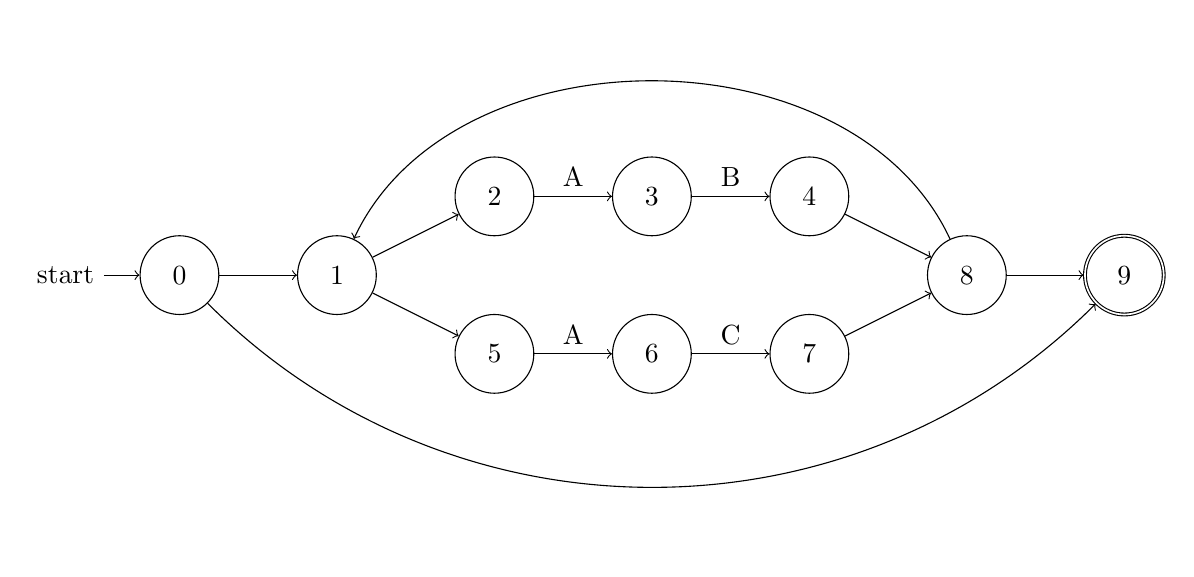
\begin{tikzpicture}
                        \node[state, minimum size=1cm, initial] (0) at (0, 0) {$0$};
                        \node[state, minimum size=1cm] (1) at (2, 0) {$1$};
                        \node[state, minimum size=1cm] (2) at (4, 1) {$2$};
                        \node[state, minimum size=1cm] (3) at (6, 1) {$3$};
                        \node[state, minimum size=1cm] (4) at (8, 1) {$4$};
                        \node[state, minimum size=1cm] (5) at (4, -1) {$5$};
                        \node[state, minimum size=1cm] (6) at (6, -1) {$6$};
                        \node[state, minimum size=1cm] (7) at (8, -1) {$7$};
                        \node[state, minimum size=1cm] (8) at (10, 0) {$8$};
                        \node[state, minimum size=1cm, accepting] (9) at (12, 0) {$9$};

                        \draw
                        (0) edge[->] (1)
                        (0) edge[->, bend right=45] (9)
                        (1) edge[->] (2)
                        (1) edge[->] (5)
                        (2) edge[->, above] node{A} (3)
                        (3) edge[->, above] node{B} (4)
                        (4) edge[->] (8)
                        (5) edge[->, above] node{A} (6)
                        (6) edge[->, above] node{C} (7)
                        (7) edge[->] (8)
                        (8) edge[->] (9)
                        (8) edge[->, bend right=65] (1);
                    \end{tikzpicture}
                \end{center}
                The DFA is then generated as follows (note that in lieu of writing out the entire closure, I use a single character, however it's best to write out the entire thing);
                \begin{enumerate}[1.]
                    \itemsep0em
                    \item create a state for 0 with its closure (01259), let it be $p$
                    \item looking at the states within $p$, we see that the ones with non-$\epsilon$-transitions are 2 and 5, both with transitions with label 'A', to 3 and 6 respectively
                    \item create a state for 3 and 6, with its closure (36), let it be $q$
                    \item looking at the states within $q$, we see that the ones with non-$\epsilon$-transitions are both 3 and 6, with transitions 'B' to 4, and 'C' to 7 respectively
                    \item create a state for 4, with its closure (124589), let it be $r$
                    \item looking at the states within $r$, we see that the ones with non-$\epsilon$-transitions are 2 and 5 - however we have already seen  this, it goes to the state $q$
                    \item create a state for 7, with its closure (125789), let it be $s$
                    \item $s$ also goes to $q$ for the same reasoning as above
                    \item all the states that contain 9 are now marked as accepting states, which are $p$, $r$, $s$
                \end{enumerate}
                This gives us the following DFA
                \begin{center}
                    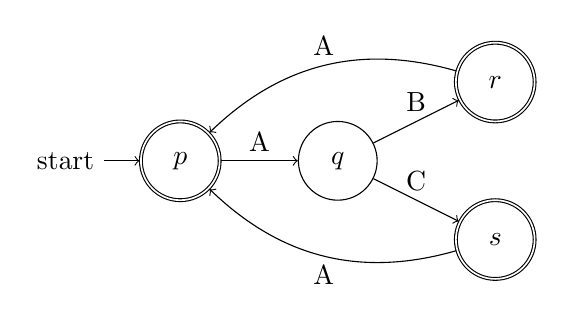
\begin{tikzpicture}
                        \node[state, minimum size=1cm, initial, accepting] (p) at (0, 0) {$p$};
                        \node[state, minimum size=1cm] (q) at (2, 0) {$q$};
                        \node[state, minimum size=1cm, accepting] (r) at (4, 1) {$r$};
                        \node[state, minimum size=1cm, accepting] (s) at (4, -1) {$s$};

                        \draw
                        (p) edge[->, above] node{A} (q)
                        (q) edge[->, above] node{B} (r)
                        (q) edge[->, above] node{C} (s)
                        (r) edge[->, above, bend right=30] node{A} (p)
                        (s) edge[->, below, bend left=30] node{A} (p);
                    \end{tikzpicture}
                \end{center}
            \subsubsection*{LR (Bottom-up) Parsing}
                The rules in the context free grammar exist as $~R~ \to ~(R|t)*~$, where ~R~ is a rule, and ~t~ is a token.
                Therefore rules are represented as some arbitrary combination of rules and tokens (thus supporting recursion, unlike regular expressions).
                The goal of a parser is to convert a sequence of tokens into an AST (or parse tree).
                In the case of the AST we can discard tokens that are simply syntactic sugar, as the structure of the program is represented in the tree.
                \medskip

                Note that we need to look at subsets of CFGs, as they can be cubic ($O(n^3)$) to parse in the worst case, and we want to consider the largest subsets which take $O(n)$.
                The types we consider are as follows (node that $\text{LL}(n) \subseteq \text{LR}(n)$, therefore LR parsers are more powerful);
                \begin{itemize}
                    \itemsep0em
                    \item LL($k$) \hfill \textbf{l}eft to right scanning, with $k$ token look-ahead, and \textbf{l}eft-most derivation
                        \subitem top-down, as it builds the AST from the root nodes to the leaf nodes
                    \item LR($k$) \hfill \textbf{l}eft to right scanning, with $k$ token look-ahead, and \textbf{r}ight-most derivation
                        \subitem bottom-up, as it builds the AST from the leaf nodes to the root node
                \end{itemize}
                We will be first looking at LR(0), then LR(1), and then finally LALR(1).
                \medskip

                Starting with LR(0), it doesn't need the token for a reduce.
                An LR(0) item is a "rule" with a dot ($\bullet$) at some position in the right hand side.
                An item indicates how much of a rule we've seen.
                For example, the item $~E~ \to ~E +~ \lrbt ~int~$ indicates that we've seen an expression, followed by a plus, and we are hoping to see an integer to complete the item.
                This means that LR(0) items represent the steps to recognise the RHS of a given production.
                \medskip

                For example, we can look at the rules for $~X~ \to ~ABC~$;
                \begin{align*}
                    ~X~ & \to \lrbt ~ABC~ & \text{initial item} \\
                    ~X~ & \to ~A~ \lrbt ~BC~ \\
                    ~X~ & \to ~AB~ \lrbt ~C~ \\
                    ~X~ & \to ~ABC~ \lrbt & \text{complete item} \\
                \end{align*}
                $$~X~ \to \underbrace{~AB~}_\text{seen} \bullet \hspace{-0.4cm} \overbrace{~C~}^\text{hope to see}$$
                These items are used as states of a finite automaton to maintain information about the progress of a shift-reduce parser.
                We can build an NFA from these items as follows (and then build a DFA with subset construction).
                Working with the single rule $~X~ \to ~A~ \lrbt ~BC~$, we add the following transition;
                \begin{center}
                    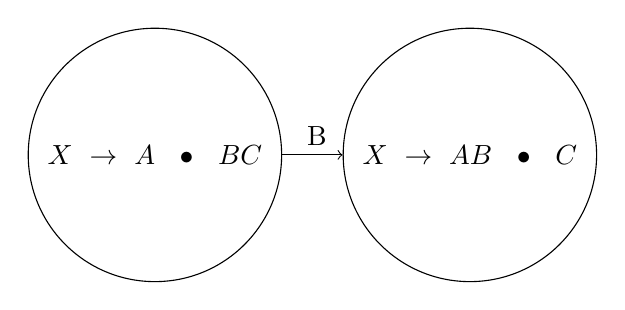
\begin{tikzpicture}
                        \node[state] (0) at (0, 0) {$~X~ \to ~A~ \lrbt ~BC~$};
                        \node[state] (1) at (4, 0) {$~X~ \to ~AB~ \lrbt ~C~$};
                        \draw (0) edge[->, above] node{~B~} (1);
                    \end{tikzpicture}
                \end{center}
                Additionally, if $~B~$ is non-terminal, such that $~B~ \to ~D~ \bnfsep ~E~ \bnfsep \cdots$, add an $\epsilon$-transition for each rule;
                \begin{center}
                    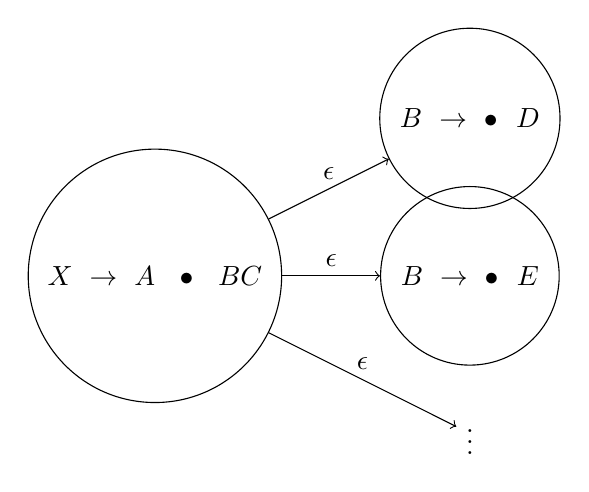
\begin{tikzpicture}
                        \node[state] (0) at (0, 0) {$~X~ \to ~A~ \lrbt ~BC~$};
                        \node[state] (1) at (4, 2) {$~B~ \to \lrbt ~D~$};
                        \node[state] (2) at (4, 0) {$~B~ \to \lrbt ~E~$};
                        \node (3) at (4, -2) {$\vdots$};
                        \draw
                        (0) edge[->, above] node{$\epsilon$} (1)
                        (0) edge[->, above] node{$\epsilon$} (2)
                        (0) edge[->, above] node{$\epsilon$} (3);
                    \end{tikzpicture}
                \end{center}
                We also need to add a start rule, with symbol to indicate the end of input ~\$~ (it is implied if omitted).
                For example, given the grammar
                \begin{center}
                    $~E~ \to ~E '+' int~ \bnfsep ~int~$
                \end{center}
                We'd add a rule $~E'~ \to ~E \$~$.
                This therefore has a total of 8 items;
                \begin{align*}
                    ~E'~ & \to \lrbt ~E~ & \text{initial item} \\
                    ~E'~ & \to ~E~ \lrbt & \text{complete / reduce item} \\
                    ~E~ & \to \lrbt ~E + int~ & \text{initial item} \\
                    ~E~ & \to ~E~ \lrbt ~+ int~ \\
                    ~E~ & \to ~E +~ \lrbt ~int~ \\
                    ~E~ & \to ~E + int~ \lrbt & \text{complete item} \\
                    ~E~ & \to \lrbt ~int~ & \text{initial item} \\
                    ~E~ & \to ~int~ \lrbt & \text{complete item}
                \end{align*}
            \subsubsection*{Chomsky Hierarchy}
                In the following, ~R~ is a non-terminal (name of a rule), ~t~ is a sequence of terminals, and $\alpha, \beta, \varphi$ are sequences of terminals and non-terminals.
                \begin{enumerate}[{type X:}]
                    \itemsep0em
                    \item[type 3:] $~R~ \to ~t~$ \hfill regular grammars (DFA)
                    \item[type 2:] $~R~ \to \alpha$ \hfill context free grammars (pushdown automata)
                    \item[type 1:] $\alpha~R~\beta \to \alpha \varphi \beta$ \hfill context sensitive grammars (linear bounded automata)
                    \item[type 0:] $\alpha \to \beta$ \hfill unrestricted grammars
                \end{enumerate}
        \subsection*{22nd January 2020}
            \subsubsection*{DFA to LR(0) Parsing Table}
                From the LR(0) items, it's fairly straightforward to determine the $\epsilon$-closures, therefore the DFA can be constructed directly (however it can also be constructed with subset construction from a NFA).
                Continuing on with the simple expression example from last lecture, we can construct the DFA with the following rules in each state;
                \begin{align*}
                    \intertext{state 0:}
                    ~E'~ & \to \lrbt ~E~ \\
                    ~E~ & \to \lrbt ~E + int~ \\
                    ~E~ & \to \lrbt ~int~
                    \intertext{state 1:}
                    ~E'~ & \to ~E~ \lrbt \\
                    ~E~ & \to ~E~ \lrbt ~+ int~
                    \intertext{state 2:}
                    ~E~ & \to ~E +~ \lrbt ~int~
                    \intertext{state 3:}
                    ~E~ & \to ~E + int~ \lrbt
                    \intertext{state 4:}
                    ~E~ & \to ~int~ \lrbt
                \end{align*}
                \begin{center}
                    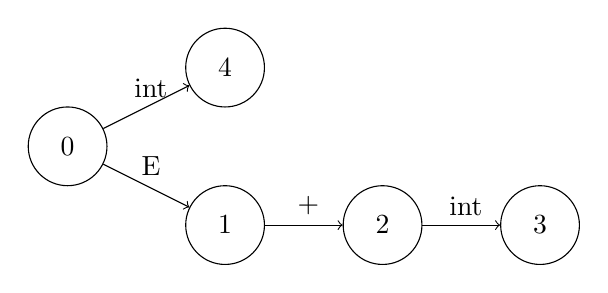
\begin{tikzpicture}
                        \node[state, minimum size=1cm] (0) at (0, 0) {0};
                        \node[state, minimum size=1cm] (4) at (2, 1) {4};
                        \node[state, minimum size=1cm] (1) at (2, -1) {1};
                        \node[state, minimum size=1cm] (2) at (4, -1) {2};
                        \node[state, minimum size=1cm] (3) at (6, -1) {3};
                        \draw
                        (0) edge[->, above] node{~E~} (1)
                        (0) edge[->, above] node{~int~} (4)
                        (1) edge[->, above] node{~+~} (2)
                        (2) edge[->, above] node{~int~} (3);
                    \end{tikzpicture}
                \end{center}
                Converting from this to a parsing table, we follow these rules;
                \begin{itemize}
                    \itemsep0em
                    \item for each terminal transition $~X~ \xrightarrow{~T~} ~Y~$ add ~P[X, T] = sY~ (shift ~Y~)
                        \subitem "move from state ~X~ to state ~Y~"
                    \item for each non-terminal transition $~X~ \xrightarrow{~N~} ~Y~$ add ~P[X, N] = gY~ (goto ~Y~)
                    \item for each state ~X~ containing $~R'~ \to \cdots \lrbt$ add ~P[X, \$] = a~ (accept)
                        \subitem this corresponds to the auxiliary rule, when we are done parsing
                    \item for each state ~X~ which contains a $~R~ \to \cdots \lrbt$ add ~P[X, T] = rn~ (reduce) for every terminal ~T~, where ~n~ is ~R~'s rule number
                        \subitem the number does not correspond to a state, it instead corresponds to a rule number, by looking at the corresponding rule, we know how many items need to be popped off the stack and reduced
                \end{itemize}
                For the DFA above, we can represent it as the following LR(0) parsing table;
                Anything left blank is considered an error.
                \begin{center}
                    \begin{tabular}{|c|c|c|c|c|}
                        \hline
                        \multirow{2}{*}{state} & \multicolumn{3}{c}{action} & goto \\
                        \cline{2-5}
                        & ~int~ & ~+~ & ~\$~ & ~E~ \\
                        \hline
                        0 & ~s4~ & & & ~g1~ \\
                        1 & & ~s2~ & ~a~ & \\
                        2 & ~s3~ & & & \\
                        4 & ~r1~ & ~r1~ & ~r1~ & \\
                        3 & ~r2~ & ~r2~ & ~r2~ & \\
                        \hline
                    \end{tabular}
                \end{center}
            \subsubsection*{Model of an LR Parser}
                Assuming all the states are integers, we can approach the LR parser as follows;
                \begin{enumerate}[1.]
                    \itemsep0em
                    \item push state 0 onto the stack
                    \item repeatedly decide what to do next depending on the top of the stack and the current character (~switch P[S[top], curr]~)
                        \begin{itemize}
                            \itemsep0em
                            \item shift ~n~ \hfill push the state ~n~ onto the stack, and go to the next token
                            \item reduce ~n~ \hfill (complex)
                                \begin{itemize}
                                    \itemsep0em
                                    \item remove ~K~ elements off the stack, where ~K~ is the length of the RHS of \textbf{rule} ~n~
                                    \item push ~P[S[top], L]~ where ~L~ is the LHS of \textbf{rule} ~n~; this essentially looks at the state it was in before, and performs the "goto"
                                        \subitem in our example if we reduced to an ~E~, state 0 is most likely on the top of the stack, and therefore it goes to state 1
                                    \item generate an AST node with this data for the rule
                                \end{itemize}
                            \item accept
                            \item error \hfill report an error
                            \item goto ~n~ \hfill not directly selected, looked up in reduce case
                        \end{itemize}
                \end{enumerate}
            \subsubsection*{FIRST and FOLLOW Sets}
                While it is possible to formally write out the algorithm for deriving the sets, it's easier to do it by intuition.
                \begin{itemize}
                    \itemsep0em
                    \item FIRST set
                        \medskip

                        The FIRST set of a terminal is itself.
                        However, the FIRST set for a rule is anything that can begin the derivation for such that particular rule.
                        This set is constructed recursively, by looking through the FIRST sets of the first item of the LHS of each rule.
                        However, note that because we are generating a set, we can stop when we encounter something we've already checked, as it wouldn't be added anyways.
                        Let the rule be ~R~, let ~X~ be an arbitrary rule, and let ~t~ be a terminal;
                        \begin{itemize}
                            \itemsep0em
                            \item $~R~ \to ~t~ \cdots$ \hfill starts with a terminal
                                \subitem add ~t~ to the FIRST set of ~R~
                            \item $~R~ \to ~X~ \cdots$ \hfill starts with a non-terminal
                                \subitem add the FIRST set of ~X~, this can lead to recursion (which can be dealt with)
                        \end{itemize}
                    \item FOLLOW set
                        \medskip

                        The FOLLOW set of a rule is something that can come after it.
                        The intuition in this is to look at how it is used in the RHS of productions.
                        On the RHS, there are three cases (or more, I could be wrong), let the rule be ~R~, let ~X~, ~Y~ be arbitrary rules, and let ~t~ be a terminal;
                        \begin{itemize}
                            \itemsep0em
                            \item $~X~ \to \cdots ~R~$ \hfill at the end of a rule
                                \subitem add the FOLLOW set of ~X~, as anything following ~X~ could follow ~R~
                            \item $~X~ \to \cdots ~R t~ \cdots$ \hfill followed by a terminal
                                \subitem add ~t~ to the FOLLOW set of ~R~
                            \item $~X~ \to \cdots ~R Y~ \cdots$ \hfill followed by a non-terminal / rule
                                \subitem add the FIRST set of ~Y~, as anything that could start a derivation of ~Y~ could follow ~X~
                        \end{itemize}
                        Note that the same intuition on recursion applies.
                        For example, in the first case, if ~R~ = ~X~, then the FOLLOW set of ~R~ needs the FOLLOW set of ~R~, but there's no point in doing this.
                \end{itemize}
                It's also important to consider the case where it can be $\epsilon$.
        \subsection*{24th January 2020}
            \subsubsection*{Weights}
                In the grammar, we've defined expressions to be right associative, hence it is a right growing tree.
                This requires more registers if we evaluate the left side first, as we need to retain this result for the next calculation.
                This can be shown in the example below, for the evaluation of $1 + 2 + 3$, with the left tree begin left associative $(1 + 2) + 3$, and the right tree being right associative $1 + (2 + 3)$ - note that the former uses 2 registers, whereas the latter uses 3.
                \begin{center}
                    \hfill
                    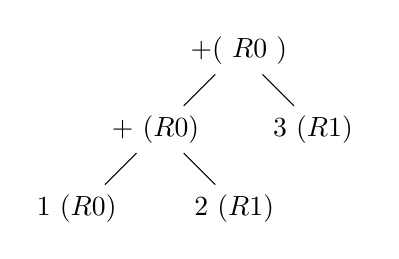
\begin{tikzpicture}
                        \node (p1) at (0, 0) {$+ (~R0~)$};
                        \node (p2) at (-1, -1) {$+ ~(R0)~$};
                        \node (1) at (-2, -2) {$1 ~(R0)~$};
                        \node (2) at (0, -2) {$2 ~(R1)~$};
                        \node (3) at (1, -1) {$3 ~(R1)~$};

                        \draw
                        (p1) -- (p2)
                        (p1) -- (3)
                        (p2) -- (1)
                        (p2) -- (2);
                    \end{tikzpicture}
                    \hfill
                    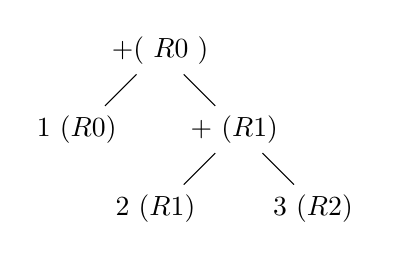
\begin{tikzpicture}
                        \node (p1) at (0, 0) {$+ (~R0~)$};
                        \node (p2) at (1, -1) {$+ ~(R1)~$};
                        \node (1) at (-1, -1) {$1 ~(R0)~$};
                        \node (2) at (0, -2) {$2 ~(R1)~$};
                        \node (3) at (2, -2) {$3 ~(R2)~$};

                        \draw
                        (p1) -- (1)
                        (p1) -- (p2)
                        (p2) -- (2)
                        (p2) -- (3);
                    \end{tikzpicture}
                    \hfill \phantom{}
                \end{center}
                The general idea for this is to first evaluate the subexpression that requires more registers.
                For example, let there be a binary operator with operands $e_1$ and $e_2$, needing $L$ registers, and $R$ registers respectively.
                If we choose to evaluate $e_1$ first, then we require $L$ registers, and $R + 1$ registers - this is because in the evaluation of $e_2$, we need to use $R$ registers, as well as maintaining the result of $e_1$.
                Therefore, the cost (in registers) for evaluating $e_1$ first is $c_1 = \max \{ L, R + 1 \}$.
                Under similar reasoning, the cost of evaluating $e_2$ first is $c_2 = \max \{ L + 1, R \}$.
                Therefore, assuming we always choose the optimal subtree in terms of registers, we have the overall cost of evaluating the binary operation is $\min \{ c_1, c_2 \}$.
                We can represent the weights as follows;
                \begin{lstlisting}
                    weight :: Exp -> Int
                    weight (Const _) = 1
                    weight (Ident _) = 1
                    weight (Binop _ e1 e2) = min c1 c2
                      where
                        c1 = max (weight e1) (weight e2) + 1
                        c2 = max (weight e1) + 1 (weight e2)
                \end{lstlisting}
                However, when we specify the target registers (naively) we have one of two issues;
                \begin{itemize}
                    \itemsep0em
                    \item it stores the result of ~e2~ into ~r~, and ~e1~ into ~(r + 1)~, when ~e2~ is evaluated first, this leads to issues with operators that aren't commutative
                    \item trying to fix the above, and storing ~e2~ into ~(r + 1)~, then evaluating ~e1~ into ~r~ - the evaluation of ~e1~ may modify the contents of ~(r + 1)~, hence overwriting the result of ~e2~
                \end{itemize}
                The fix is to give the expression translation function a list of registers it's able to use.
                The result should be stored into the first register in that list.
                \begin{lstlisting}
                    transExp :: Exp -> [Register] -> [Instruction]
                    transExp (Const n) (dst:_) = [LoadImm dst n]
                    transExp (Ident x) (dst:_) = [LoadAbs dst x]
                    transExp (Binop op e1 e2) (dst:nxt:rest)
                      | weight e1 > weight e2 =
                          transExp e1 (dst:nxt:rest) ++
                          transExp e2 (nxt:rest) ++
                          transBinop op dst nxt
                      | otherwise =
                          transExp e1 (dst:nxt:rest) ++
                          transExp e2 (nxt:rest) ++
                          transBinop op dst nxt
                \end{lstlisting}
                However, this can be further optimised by using more advanced instructions such as doing immediate addressing whenever possible.
                The translator can use pattern-matching to detect these cases.
                \medskip

                The worst case for this is a perfectly balanced tree.
                This is because if it is unbalanced, then we can always choose a more optimal side.
                When there are $k$ operators, and $k - 1$ intermediate values, the number of registers is the depth of the tree ($\ceil{\log_2(k)}$).
                This means that with $N$ registers, we can support expressions with up to $2^N$ operators.
                \medskip

                Note that the algorithm above can lead to issues when working with side effecting expressions, as the order of execution is important.
                For example, ~(x)+(x++)~ is different from ~(x++)+(x)~.
            \subsubsection*{Function Calls}
                At the function call, registers may already be in use, and therefore those will need to be saved.
                Note that the address of the next instruction also has to be saved onto the stack, for the function to return to the correct place (notice how the control paths are coloured).
                Consider the example below, where $~body~_~0~$ requires the set of registers $M$, $~body~_~1~$ requires set $N$, and $~body~_~F~$ requires set $P$.
                \begin{center}
                    \begin{tikzpicture}[y=0.6cm]
                        \node[anchor=west] (b0) at (0, 0) {$~body~_~0~$};
                        \node[anchor=west] (j1) at (0, -1) {$~Jsr F~$};
                        \node[anchor=west] (b1) at (0, -2) {$~body~_~1~$};
                        \node[anchor=west] (j2) at (0, -3) {$~Jsr F~$};
                        \node[anchor=west] (b2) at (0, -4) {$~body~_~2~$};
                        \node[anchor=west] (f) at (3, 0) {$~F:~$};
                        \node[anchor=west] (bf) at (3.5, -1) {$~body~_~F~$};
                        \node[anchor=west] (r) at (3.5, -2) {$~ret~$};

                        \draw[blue]
                        (j1.east) edge[->] (f.west)
                        (r.west) edge[->] (b1.east);

                        \draw[red]
                        (j2.east) edge[->] (f.west)
                        (r.west) edge[->] (b2.east);
                    \end{tikzpicture}
                \end{center}
                There are two conventions (and a hybrid of the two) for saving registers with regards to calls;
                \begin{itemize}
                    \itemsep0em
                    \item \textbf{caller-saved}
                        \medskip

                        Before the instruction ~Jsr F~ is executed (after $~body~_~0~$), it saves the intersection of registers currently in use, and registers that the function will use $(M \cap P)$.
                        After the function returns, it restores $(M \cap P)$.
                    \item \textbf{callee-saved}
                        \medskip

                        Since the callee doesn't know which jump it's coming from, it has to save everything that \textbf{might} be in use.
                        Before $~body~_~F~$ is executed, it saves the set of registers $(M \cup N) \cap P$, and then restores it before returning.
                \end{itemize}
            \subsubsection*{Optimising Compilers}
                While the Sethi-Ullman algorithm we followed is fast, and very easy to test, it's essentially a tree walk.
                Therefore it doesn't take into context what it's translating (other than the small optimisation we used to determine weights),
                Currently, in our implementation, we don't use registers to carry values between states, and only use them to store intermediate values for computation.
                An optimising compiler can have named variables in the register, with no reference to the main memory, therefore being much faster.
                Note that Sethi-Ullman is optimal in trees that have no shared subtrees.
            \subsubsection*{Graph Colouring}
                An obvious optimisation of the code below;
                \begin{lstlisting}
                    a1 := b1 + s * k
                    a2 := b2 + s * k
                \end{lstlisting}
                would be compute the value of ~s * k~ into a temporary variable (stored in a register) and use it for both expressions;
                \begin{lstlisting}
                    t  := s * k
                    a1 := b1 + t
                    a2 := b2 + t
                \end{lstlisting}
                We need to consider all variables on equal terms (not just ones defined by the programmer) - including intermediate values during computation.
                \medskip

                This can be achieved by doing the following;
                \begin{enumerate}[(1)]
                    \itemsep0em
                    \item perform a simple tree walk to generate intermediate code where temporary values are saved in named locations (three address code - looks similar to assembly but with infinite registers)
                    \item construct an interference graph, where the nodes are temporary locations, and an arc between two nodes represents an overlap in live ranges (if they must be stored simultaneously)
                    \item colour the graph, with each register being its own colour - no connected nodes can have the same register
                \end{enumerate}
                This is very straightforward in the case of straight line code, as we simply consider the live-in to be the first use of the value (when it is first declared), and the live-out to be the last use.
                Note that the LHS and RHS of an assignment does not count as a simultaneous use.
                \begin{lstlisting}[escapechar=!]
                    !\tikz[remember picture] \node (l1) {};!A!\tikz[remember picture] \node (ain) {};!:=!\tikz[remember picture] \node {};!e1
                    !\tikz[remember picture] \node (l2) {};!B!\tikz[remember picture] \node (bin) {};!:=!\tikz[remember picture] \node {};!e2
                    !\tikz[remember picture] \node (l3) {};!...
                    !\tikz[remember picture] \node (l4) {};!... B ...
                    !\tikz[remember picture] \node (l5) {};!C!\tikz[remember picture] \node (cin) {};!:=!\tikz[remember picture] \node (boutp) {};!A + B!\tikz[remember picture] \node (bout) {};!
                    !\tikz[remember picture] \node (l6) {};!...
                    !\tikz[remember picture] \node (l7) {};!D!\tikz[remember picture] \node (din) {};!:=!\tikz[remember picture] \node (aoutp) {};!A * 5!\tikz[remember picture] \node (aout) {};!
                    !\tikz[remember picture] \node (l8) {};!... D ...!\tikz[remember picture] \node (dout) {};!
                    !\tikz[remember picture] \node (l9) {};!... C ...!\tikz[remember picture] \node (cout) {};!
                \end{lstlisting}
                \begin{tikzpicture}[remember picture, overlay]
                    \draw[violet, dashed, name path=alive]
                    (ain.south) -- (ain.north) -- (l1.north) -- (l7.north) -- (aoutp.north) -- (aoutp.south) -- (aout.south) |- cycle;

                    \draw[blue, dashed, name path=blive]
                    (bin.south) -- (bin.north) -- (l2.north) -- (l5.north) -- (boutp.north) -- (boutp.south) -- (bout.south) |- cycle;

                    \draw[red, dashed, name path=clive]
                    (cin.south) -- (cin.north) -- (l5.north) -- (l9.south) -- (cout.south) |- cycle;

                    \draw[olive, dashed, name path=dlive]
                    (din.south) -- (din.north) -- (l7.north) -- (l8.south) -- (dout.south) |- cycle;
                \end{tikzpicture}
                This gives the following interference graph, and the result of the colouring;
                \begin{center}
                    \hfill
                    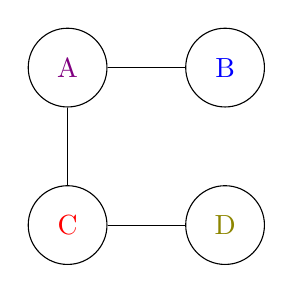
\begin{tikzpicture}
                        \node[state, minimum size=1cm] (a) at (0, 0) {\violet{~A~}};
                        \node[state, minimum size=1cm] (b) at (2, 0) {\blue{~B~}};
                        \node[state, minimum size=1cm] (c) at (0, -2) {\red{~C~}};
                        \node[state, minimum size=1cm] (d) at (2, -2) {\textcolor{olive}{~D~}};

                        \draw
                        (a) -- (b)
                        (a) -- (c)
                        (c) -- (d);
                    \end{tikzpicture}
                    \hfill
                    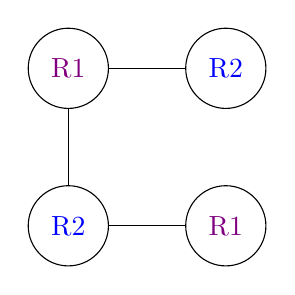
\begin{tikzpicture}
                        \node[state, minimum size=1cm] (a) at (0, 0) {\violet{~R1~}};
                        \node[state, minimum size=1cm] (b) at (2, 0) {\blue{~R2~}};
                        \node[state, minimum size=1cm] (c) at (0, -2) {\blue{~R2~}};
                        \node[state, minimum size=1cm] (d) at (2, -2) {\violet{~R1~}};

                        \draw
                        (a) -- (b)
                        (a) -- (c)
                        (c) -- (d);
                    \end{tikzpicture}
                    \hfill \phantom{}
                \end{center}
        \subsection*{27th January 2020}
            \subsubsection*{LR(1) Items}
                An LR(1) item is a pair consisting of an LR(0) item, and a lookahead token ~t~.
                The process for a terminal doesn't change much;
                \begin{center}
                    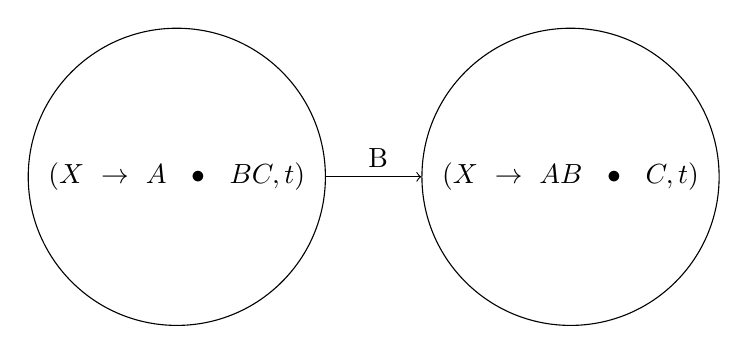
\begin{tikzpicture}
                        \node[state] (0) at (0, 0) {$~(X~ \to ~A~ \lrbt ~BC, t)~$};
                        \node[state] (1) at (5, 0) {$~(X~ \to ~AB~ \lrbt ~C, t)~$};
                        \draw (0) edge[->, above] node{~B~} (1);
                    \end{tikzpicture}
                \end{center}
                However, if ~B~ is a rule, then for each rule in the form $~B~ \to ~D~$, we add an $\epsilon$-transition for every token ~u~ in FIRST(~Ct~), we add a transition if and only if the string following ~B~ is derivable from ~Ct~.
                \begin{center}
                    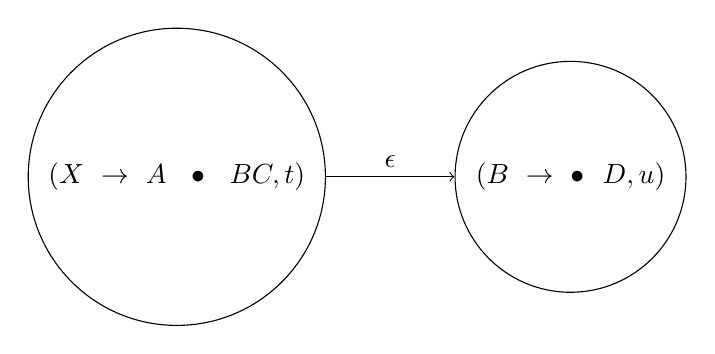
\begin{tikzpicture}
                        \node[state] (0) at (0, 0) {$~(X~ \to ~A~ \lrbt ~BC, t)~$};
                        \node[state] (1) at (5, 0) {$~(B~ \to \lrbt ~D, u)~$};
                        \draw (0) edge[->, above] node{$\epsilon$} (1);
                    \end{tikzpicture}
                \end{center}
                The auxiliary item $~(X'~ \to \lrbt ~X, \$)~$ is also added to start the construction of the parsing table.
                The reduction is only done if the current token matches ~t~.
                Consider the following grammar (not written with the vertical separation), and the states of the DFA;
                \begin{align*}
                    ~S'~ & \to ~\underline{S} \$~ \\
                    ~S~ & \to ~id~ & & ~r1~ \\
                    ~S~ & \to ~\underline{V} = \underline{E}~ & & ~r2~ \\
                    ~V~ & \to ~id~ & & ~r3~ \\
                    ~E~ & \to ~\underline{V}~ & & ~r4~ \\
                    ~E~ & \to ~int~ & & ~r5~
                    \intertext{state 0:}
                    ~S'~ & \to \lrbt ~\underline{S}, \$~ & \text{starting state} &\ [1] \\
                    ~S~ & \to \lrbt ~id, \$~ & \text{derived from non-terminal in (1)} &\ [2] \\
                    ~S~ & \to \lrbt ~\underline{V} = \underline{E}, \$~ & \text{derived from non-terminal in (1)} &\ [3] \\
                    ~V~ & \to \lrbt ~id, =~ & \text{derived from non-terminal in (3)} &\ [4]
                    \intertext{state 1:}
                    ~S'~ & \to ~\underline{S}~ \lrbt ~, \$~ & \text{shift from (1)} &\ [5]
                    \intertext{state 2:}
                    ~S~ & \to ~id~ \lrbt ~, \$~ & \text{shift from (2)} &\ [6] \\
                    ~V~ & \to ~id~ \lrbt ~, =~ & \text{shift from (4)} &\ [7]
                    \intertext{state 3:}
                    ~S~ & \to ~\underline{V}~ \lrbt ~= \underline{E}, \$~ & \text{shift from (3)} &\ [8]
                    \intertext{state 4:}
                    ~S~ & \to ~\underline{V} =~ \lrbt ~\underline{E}, \$~ & \text{shift from (8)} &\ [9] \\
                    ~E~ & \to \lrbt ~int, \$~ & \text{derived from non-terminal in (9)} &\ [10] \\
                    ~E~ & \to \lrbt ~\underline{V}, \$~ & \text{derived from non-terminal in (9)} &\ [11] \\
                    ~V~ & \to \lrbt ~id, \$~ & \text{derived from non-terminal in (11)} &\ [12]
                    \intertext{state 5:}
                    ~S~ & \to ~\underline{V} = \underline{E}~ \lrbt ~, \$~ & \text{shift from (8)} &\ [13]
                    \intertext{state 6:}
                    ~E~ & \to ~int~ \lrbt ~, \$~ & \text{shift from (10)} &\ [14]
                    \intertext{state 7:}
                    ~E~ & \to ~\underline{V}~ \lrbt  ~, \$~ & \text{shift from (11)} &\ [15]
                    \intertext{state 8:}
                    ~V~ & \to ~id~ \lrbt ~, \$~ & \text{shift from (12)} &\ [16]
                \end{align*}
                \begin{center}
                    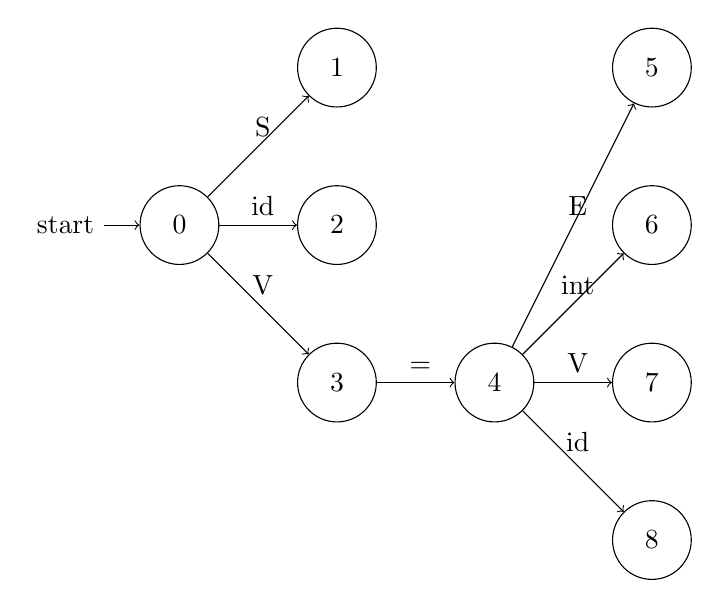
\begin{tikzpicture}
                        \node[state, minimum size=1cm, initial] (0) at (0, 0) {$0$};
                        \node[state, minimum size=1cm] (1) at (2, 2) {$1$};
                        \node[state, minimum size=1cm] (2) at (2, 0) {$2$};
                        \node[state, minimum size=1cm] (3) at (2, -2) {$3$};
                        \node[state, minimum size=1cm] (4) at (4, -2) {$4$};
                        \node[state, minimum size=1cm] (5) at (6, 2) {$5$};
                        \node[state, minimum size=1cm] (6) at (6, 0) {$6$};
                        \node[state, minimum size=1cm] (7) at (6, -2) {$7$};
                        \node[state, minimum size=1cm] (8) at (6, -4) {$8$};
                        \draw
                        (0) edge[->, above] node{~S~} (1)
                        (0) edge[->, above] node{~id~} (2)
                        (0) edge[->, above] node{~V~} (3)
                        (3) edge[->, above] node{~=~} (4)
                        (4) edge[->, above] node{~E~} (5)
                        (4) edge[->, above] node{~int~} (6)
                        (4) edge[->, above] node{~V~} (7)
                        (4) edge[->, above] node{~id~} (8);
                    \end{tikzpicture}
                \end{center}
                This is represented in the following parsing table - note that the reduce state now only happens when it matches ~t~;
                \begin{center}
                    \begin{tabular}{|c|c|c|c|c|c|c|c|}
                        \hline
                        \multirow{2}{*}{state} & \multicolumn{4}{c|}{action} & \multicolumn{3}{c|}{goto} \\
                        \cline{2-8}
                        & ~id~ & ~int~ & ~=~ & ~\$~ & ~\underline{E}~ & ~\underline{V}~ & ~\underline{S}~ \\
                        \hline
                        0 & ~s2~ & & & & & ~g3~ & ~g1~ \\
                        1 & & & & ~a~ & & & \\
                        2 & & & ~r3~ & ~r1~ & & & \\
                        3 & & & ~s4~ & & & & \\
                        4 & ~s8~ & ~s6~ & & & ~g5~ & ~g7~ & \\
                        5 & & & & ~r2~ & & & \\
                        6 & & & & ~r5~ & & & \\
                        7 & & & & ~r4~ & & & \\
                        8 & & & & ~r3~ & & & \\
                        \hline
                    \end{tabular}
                \end{center}
            \subsubsection*{LALR(1)}
                In reality, LR(1) parsers don't really exist.
                We optimise LR(1) by merging LR(1) items that have the same LR(0) item, but different lookaheads into a single LALR(1) item that has the LR(0) item and the combined set of lookaheads.
                For example, we can combine these states;
                \begin{align*}
                    \intertext{[LR(1)] state 2:}
                    ~X~ & \to ~\underline{E}~ \lrbt ~T, =~ \\
                    ~V~ & \to ~id~ \lrbt ~, +~
                    \intertext{[LR(1)] state 3:}
                    ~X~ & \to ~\underline{E}~ \lrbt ~T, \$~ \\
                    ~V~ & \to ~id~ \lrbt ~, /~
                    \intertext{[LALR(1)] state 23:}
                    ~X~ & \to ~\underline{E}~ \lrbt ~T, \{=, \$\}~ \\
                    ~V~ & \to ~id~ \lrbt ~, \{+, /\}~
                \end{align*}
                \begin{center}
                    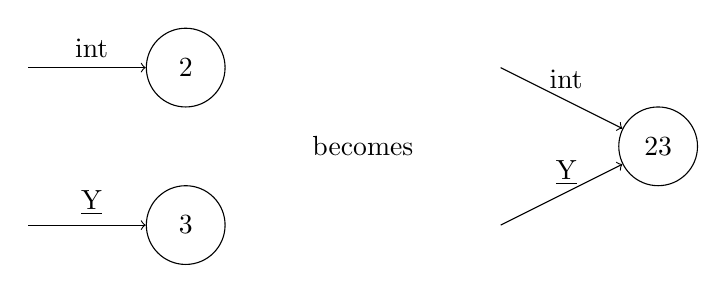
\begin{tikzpicture}
                        \node[state, minimum size=1cm] (2) at (0, 0) {$2$};
                        \node[state, minimum size=1cm] (3) at (0, -2) {$3$};
                        \draw
                        (-2, 0) edge[->, above] node{~int~} (2)
                        (-2, -2) edge[->, above] node{~\underline{Y}~} (3);

                        \node at (2.25, -1) {becomes};

                        \node[state, minimum size=1cm] (23) at (6, -1) {$23$};
                        \draw
                        (4, 0) edge[->, above] node{~int~} (23)
                        (4, -2) edge[->, above] node{~\underline{Y}~} (23);
                    \end{tikzpicture}
                \end{center}
            \subsubsection*{Ambiguity and Conflicts}
                Ambiguity can be removed by rewriting the grammar, or adding additional rules.
                For example, we can get a shift-reduce conflict when we don't know whether to reduce an item or to continue, or we can get a reduce-reduce conflict, when it could reduce to either rule;
                \begin{align*}
                    \intertext{shift-reduce conflict}
                    ~A~ & \to ~id~ & \text{can be reduced} \\
                    ~A~ & \to ~id '[' \underline{Expr} ']'~ & \text{can be shifted}
                    \intertext{reduce-reduce conflict}
                    ~Expr~ & \to ~id~ \\
                    ~Var~ & \to ~id~
                \end{align*}
                Similar to lexing, we'd normally continue shifting in the first case, and in the second case we give precedence to the first rule declared.
            \subsubsection*{Parse Trees}
                When we perform a shift, we are recognising an input and it builds a leaf node for the parse tree.
                On the other hand, when we perform a reduce, we take the leaf nodes, and put them into a parent node for the parse tree.
                However, this tree can have a lot of junk in it (thus being inconvenient to work with), and is either pruned in a separate pass to generate an abstract syntax tree (AST), or generated with instructions augmented onto the existing rules for the grammar to generate nodes as it is being parsed.
\end{document}
